\documentclass[a4paper, 9pt, landscape]{extarticle}
\usepackage[scaled=0.92]{helvet}
\usepackage{multicol}
\usepackage{calc}
\usepackage{ifthen}
\usepackage[landscape]{geometry}
\usepackage[bookmarks=false]{hyperref}

\usepackage{newtxtext} 

%for strikeout
\usepackage{ulem}

%For editing parbox
\usepackage[table]{xcolor}
%For editing itemise margins, reduce iterm separaion and list separation
\usepackage{enumitem}
% For math
\usepackage{amsmath,amsthm,amsfonts,amssymb}

%For pictures / figures
\usepackage{color,graphicx,overpic}
\graphicspath{ {./images/} }


\pdfinfo{
  /Title (notes.pdf)
  /Creator (Ger Teck)
  /Author (Ger Teck)
  /Subject ()
  /Keywords (tex)}

%% Margins for PAPER

%% Margins for A4 PAPER
\geometry{top=0.5cm,left=0.5cm,right=0.5cm,bottom=0.5cm}
\pagestyle{empty}
\newenvironment{tightcenter}{%
  \setlength\topsep{0pt}
  \setlength\parskip{0pt}
  \begin{center}
}{%
  \end{center}
}

% Redefine section commands to use less space
\makeatletter
\renewcommand{\title}{\@startsection{section}{1}{0mm}%
                                {-1ex plus -.5ex minus -.2ex}%
                                {0.5ex plus .2ex}%x
                                {\normalfont\large\bfseries}}
\renewcommand{\section}{\@startsection{subsection}{2}{0mm}%
                                {-1ex plus -.5ex minus -.2ex}%
                                {0.5ex plus .2ex}%
                                {\normalfont\normalsize\bfseries\underline}}
\renewcommand{\subsection}{\@startsection{subsubsection}{3}{0mm}%
                                {-1ex plus -.5ex minus -.2ex}%
                                {0.5ex plus .2ex}%
                                {\normalfont\small\bfseries}}
\renewcommand{\subsubsection}{\@startsection{paragraph}{4}{0mm}%
                                {-1ex plus -.5ex minus -.2ex}% Space above
                                {0.5ex plus .2ex}% POSITIVE value = Block (New line)
                                {\normalfont\footnotesize\bfseries}} % Smaller font

\makeatother
% Title becomes section
% Section becomes subsection
% Subsection becomes subsubsection


\setcounter{secnumdepth}{0}
\setlength{\parindent}{0pt}
\setlength{\parskip}{0pt plus 0.5ex}

%% this changes all items (enumerate and itemize, reduce margins)
\setlength{\leftmargini}{0.5cm}
\setlength{\leftmarginii}{0.5cm}
\setlist[itemize,1]{leftmargin=2mm,labelindent=1mm,labelsep=1mm, itemsep = 0mm, before=\justifying}
\setlist[itemize,2]{leftmargin=2mm,labelindent=0.5mm,labelsep=0.5mm, itemsep = -0.2mm, topsep=-0.2mm, before=\justifying}
%\setlist{nosep}

\usepackage[document]{ragged2e}

% -------------------------------------------------------------------------------

% START OF DOCUMENT HERE

\begin{document}
\raggedright
\footnotesize
\begin{multicols*}{3}

% multicol parameters
% These lengths are set only within the two main columns
\setlength{\columnseprule}{0pt}
\setlength{\premulticols}{1pt}
\setlength{\postmulticols}{1pt}
\setlength{\multicolsep}{2pt}
\setlength{\columnsep}{2pt}

\title{CS3217 Notes}
\centerline{github.com/gerteck}

\section{Pre-Course Readings and Resources}
Some suggested or referenced readings and watchings for the course.
\begin{itemize}
  \item \textbf{Clean Code, by Robert C Martin}, \textbf{The Mythical Man Month}, \textbf{Rework by 37signals}
\end{itemize}
Some notes for the course: CS3217 is designed to be a very intensive software engineering module, write lots of code. First 6 weeks - 4 problem sets to develop some Peggle clone by end of 6 weeks. Remaining period, work in teams of up to 4 students for the Final Project.

%https://www.facebook.com/notes/ben-leong/on-cs3216cs3217-and-elitism/10153053255577549
%https://uvents.nus.edu.sg/event/24th-steps/module/CS3217

\textbf{Final Project}: For the Final Project, allowed to build app of choice, start thinking early, see past projects for scale. Develop a good app that solves problem defined. Good to spend time to build a real product that is useful.

% Stay Hungry. Stay Foolish. (http://www.ted.com/talks/steve_jobs_how_to_live_before_you_die)
\subsubsection{Stay Hungry. Stay Foolish.}
\begin{itemize}
  \item Steve Jobs' 2005 Stanford Commencement Address. Three personal stories:
  \item \textbf{Connect the Dots}: Life events often only make sense retrospectively, trust in the journery and intuition. (Seemingly impractical knowledge may turn out useful.)
  \item \textbf{Love and What You Do}: 	Passion for work drives excellence and satisfaction, give motivation to start over and seek success.
  \item \textbf{Death as a Motivator}: Awareness of mortality helps prioritise and live authentically.
  \item \textbf{Stay Hungry, Stay Foolish}: Maintain curiosity and willingness to take risks and learn.
\end{itemize}

\subsubsection{Paul Orfalea's Keynote Address.}
\begin{itemize}
  \item Founded Kinko's (now part of FedEx). Had to overcome learning disabilities and reading writing difficulties.
  \item \textbf{Pragmatism}: Education focus on applying knowledge to real life over memorization or taking extensive notes (rip... tbf...).
  \item \textbf{Leadership}: Warned against leaders who cannot tolerate ambiguity or delegate authority, noting they risk burnout or nervous breakdown. 
  \item \textbf{Work-Life}: Balance work, love and play to avoid burnout and maintain effective leadership, anxiety and ambition are intertwined, sleep important for retention, decision making, cultivate personal happiness and relationships.
  \item Many fail to see the success around them as they are too busy or anxious.
  \item Overall, important to leverage unique strengths, focus on human relationships, balance life priorities for sustainable success.
\end{itemize}
 
% https://www.youtube.com/watch?v=ji5_MqicxSo
\subsubsection{Randy Pausch's The Last Lecture}
\begin{itemize}
  \item Persistence and creativity are key to overcoming obstacles and achieving dreams.
  \item Fun and enthusiasm fuel sustained effort and creativity.
  \item Collaboration between disciplines (art and tech) is vital for innovation.
  \item Leadership and humility, and support systems of family, mentors and colleagues are crucial for success.
\end{itemize}

\section{Problem Set 0}
Ungraded problem set to learn Swift and SWE. UI development is not the focus of this problem set.
Build a Sudoku Solver Program

\section{Lecture 1: Introduction}
\begin{itemize}
  \item CS3217: Software Engineering. CS3216: Product Development.
  \item Software Engineering: Understanding the Problem, Articulating Needs, Design, Reasoning about Correctness, Processes (Working with people, maintaining code, coping with change).
  \item Language matters not. (But it does in terms of properties and suitability.)
  \item \textbf{Problem Sets}: Learn SWE, learn Apple/Android, ccomplete app at the end, Peggle clone and achieve individual competency.
\end{itemize}

\textbf{Plan}: First 7 weeks (including recess week) - 4 problem sets, last 7 weeks - Final Project. 

\begin{itemize}
  \item \textbf{Education}: Preparing students for a job that do not yet exist in a future we cannot predict. Most valuable skill is how to learn efficiency. How to figure out what you don't know and build on what you do know to adapt to new situations and new problems.
  \item \textbf{Environment $\rightarrow$ Experience}: shaped by surroundings.
  \item \textbf{Engineering}: SWE: systematic engineering approach to software development. Engineering: use of scientific principles to design and build machines, structures, and other items.
  \item \textbf{A well engineered product}: Maintainable at its core / crux of engineering (especially for companies with software as a core product offering). Other aspects include functional, adaptable, within budget, timely, efficient.
  \item \textbf{That which cannot be maintained, will eventually die}.
  \item 'If you are not prepared to be wrong (or at least, not the best), you will never come up with anything original.' - Ken Robinson
\end{itemize}


\section{Lecture 1b: Introduction to Swift}
\begin{itemize}
  \item \textbf{Comparison}:
  \begin{itemize}
      \item \textbf{Java/C\#}: Established, traditional OOP, "Language matters not".
      \item \textbf{Kotlin/Swift}: Modern, designed from scratch, Avant-garde POP (Protocol Oriented Programming), "Language matters much".
      \item \textbf{Why Study PLanguages?}: Medium of our industry (Civil Engineering analogy). Toolchain: Xcode, Playground.
  \end{itemize}
\end{itemize}

\subsection{Swift}
\begin{itemize}
  \item \textbf{Typing}: Swift is Strongly and statically typed.
  \item \textbf{Collection Types}: Arrays, Sets, Dictionaries, \textbf{Tuples} (kind of like an immutable array that can hold differente types).
\end{itemize}

\subsection{Case Study: Swift Strings}
\begin{itemize}
  \item \textbf{Evolution of String dataType}: Swift 1: Collection $\rightarrow$ 2: Non-Collection $\rightarrow$ 4: Collection $\rightarrow$ 5: UTF-8. \textbf{Why?}
  \item \textbf{Context and definitions}: 
    \begin{itemize}
      \item \textit{ASCII} is major standard that maps 0-127 to english characters, is 1 byte (7 bits + 1 pad), can only represent English.
      \item \textit{Unicode}: Not an encoding of bits, but a giant list / map that assigns unique code points (numbers) to characters across all languages. (E.g. `A` is U+0041).
      \item \textit{UTF-8}: Modern standard, variable-width encoding of Unicode code points. Backwards compatible with ASCII (0-127 same as ASCII), uses min of 8 bits (1 byte), up to max 32 bits (4 bytes) per code point. (Note UTF-16 uses 2 or 4 bytes per code point).
    \end{itemize}
  \item \textbf{Evolution of Swift Strings}: Comparison between correctness and usability.
  \item In Swift 1, Strings as collections of characters, used UTF-16 directly, but acted as fixed-width arrays, directly jumping with subscripting chars[5] dangerous (due to variable-width encodings). 
  \item In Swift 2, String as non-collections, correct for variable-width encodings, but hard to use (no subscripting, no iteration).
  \item In Swift 4, Strings back as Collections of Characters (revisited). Balance correctness, usability with Character type (grapheme clusters). But still using UTF-16 fixed box storage.
  \item \textbf{Swift 5}: Strings as UTF-8 Collections. Improved performance and interoperability while maintaining correctness and usability.
  \item \textbf{Graphemes}: User-perceived characters. E.g., `é` can be `U+00E9` or `e` + `U+0301`. Swift handles canonical equivalence (displays identically, compares equal).
  \item \textbf{Emojis}: May not fit in single UTF-16 unit. Swift counts grapheme clusters correctly (length 1), unlike Java or C\#. In many languages, a complex Emoji is just a list of numbers. In Swift, it is a single Character.
  \item \textbf{Iterating}: (The 'No Integer Indexing' Rule): As Swift treats variable-width blobs as single characters, does not know where char 5 lives without checking preceeding characters.
\end{itemize}


\subsection{Legibility of Swift}
\begin{itemize}
  \item \textbf{Syntax}: Semicolons optional, brackets optional, braces required. Legibility focus.
  \item \textbf{Optionals}: `Type$?$` != `Type`. NOT the same as null in Java. \textit{Forced Unwrapping (!)}: Dangerous, runtime error if nil. Use \textit{Optional Chaining} instead. \texttt{a?.b?.c}. If any link is nil, result is nil. Result is always optional.
  \item \textbf{Optional Binding (if let, else)}: Unwraps into a new constant. (E.g. if let pOwner = cat.owner?.name).
  \item \textbf{Guard (guard let)}: Enforces "Golden Path" (indented scope for happy path not required). Avoid "Pyramid of Doom". Exits early if nil.
  \item \textbf{Functions}: Function parameters are labelled, which are required unless omit with \_. Parameters are constants by default, use \texttt{inout} to make mutable. Functions are also first-class citizens.
\end{itemize}

\subsection{Swift Programming Paradigms}
\begin{itemize}
  \item \textbf{Structs vs Classes}: Structures same as classes, except classes support inheritance, type cast, deinit, ref counting. So why even use structs?
  \item Structs are value types (copied on assignment), classes are reference types (reference counted). Structs on Stack, faster, Classes allocated on Heap, slower. Structs also more safe as it is copied, no shared mutable state, thread safety etc.
  \item  \textbf{When to use Structs vs Classes}:
  \begin{itemize}
      \item \textbf{Structs (Value Types)}: No inheritance, no deinit, no reference counting. Automatic member-wise initializer. Copied on assignment. \textit{Use for things that are values.}
      \item \textbf{Classes (Reference Types)}: Inheritance, reference counting, identity. \textit{Use for things that have identities}.
      \item Use Structs by default.
  \end{itemize}
  \item \textbf{Enumerations}: Group of related values of any type, first-class types, has computed properties, methods, initializers.
\end{itemize}
\centerline{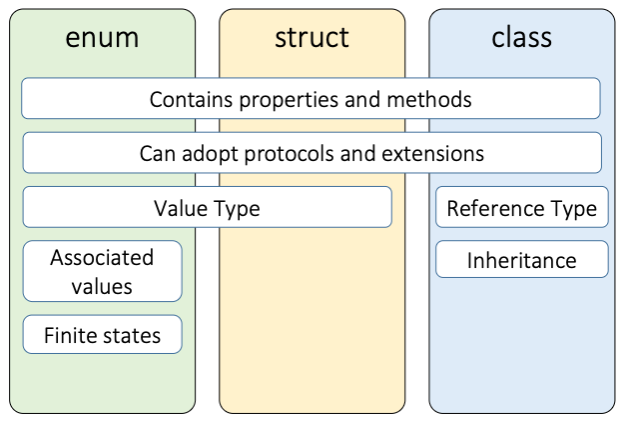
\includegraphics[width=0.5\linewidth]{SwiftConstructs.png}}

\subsection{Protocol Oriented Programming (POP)}
\begin{itemize}
  \item \textbf{Protocols}: A protocol defines a blueprint of methods, properties, and other requirements that suit a particular task or piece of functionality (Interfaces).
  \item \textbf{Extensions}: Add functionality (computed props, methods) to existing class, structure, enumeration or protocol type (even those you don't own).
\end{itemize}

\section{Lecture A: Names, Comments, Testing (Clean Code)}
\subsection{What is Clean Code?}
\begin{itemize}
\item \textbf{Definition}: Code that is easy to read, understand, and modify. 
\item Clean code is \textit{elegant, efficient}, and \textbf{does one thing well}. (Bjarne Stroustrup). Clean code reads like \textit{well-written prose}. (Grady Booch) Clean code looks like it was written by \textbf{someone who cares}. (Michael Feathers)
\item \textbf{The Boy Scout Rule}: Always leave the campground cleaner than you found it. Encourages continuous refactoring and prevents code rot.
\end{itemize}

\subsection{Meaningful Names}
\begin{itemize}
\item \textbf{Names should reveal intention}: Code should be understandable without comments. Good naming explains \textit{what} and \textit{why}.
\item \textbf{Avoid disinformation}: Do not encode container types into names (e.g. \texttt{accountList}). Focus on the \textit{concept}, not the implementation.
\item \textbf{Make meaningful distinctions}: Avoid vague variations (e.g. \texttt{data}, \texttt{data2}, \texttt{dataInfo}). Differences in names must reflect differences in meaning.
\item \textbf{Pick one word per concept}: Avoid mixing terms like \textit{controller}, \textit{manager}, \textit{director} arbitrarily. Consistency reduces cognitive load.
\item \textbf{Names should be searchable}: Single-letter names are hard to search.
(Acceptable only in small local scopes).
\item \textbf{Rule of thumb of Name Lengths}
\begin{itemize}
\item Name length should correspond to scope size.
\item Larger scope $\rightarrow$ longer, more descriptive names.
\end{itemize}

\item \textbf{Avoid mental mapping}
\begin{itemize}
\item Prefer meaningful names over short cryptic ones.
\item Readers should not need to translate names mentally.
\end{itemize}

\item \textbf{Nouns and Verbs}: \textbf{Classes}: Nouns (things). \textbf{Functions}: Verbs (actions).
\end{itemize}

\subsection{Meaningful Comments}
\begin{itemize}
\item \textbf{Why comment?}: Code should ideally be self-explanatory. Comments last resort, not a crutch.
\item \textbf{Comments do not fix bad code}: Do not comment to explain messy code. Refactor and clean the code instead.
\item \textbf{Good comments}
\begin{itemize}
\item Good comments explain \textbf{intent}.
\item Clarify unavoidable complexity (with care).
\item Warn of consequences (e.g. performance, safety).
\item Amplify the importance of non-obvious logic.
\end{itemize}

\item \textbf{Risks of clarifying comments}: Can become outdated or incorrect. Errors are hard to detect.
\item \textbf{Bad comments}: Raise more questions than they answer, repeat what code already says, or clutter the codebase. Are misleading or factually incorrect.
\item \textbf{Commented-out code}: Should be removed. Version control already preserves history.
\item \textbf{Prefer code over comments}: Replace comments with well-named variables or functions.
\end{itemize}

\subsection{Testing}
\begin{itemize}
\item \textbf{Why test?}: Prevent catastrophic failures. Increase confidence that the system behaves as intended.
\item \textbf{Case Study: Ariane 5}: Self-destructed 37 seconds after launch, due to software error of reused code of integer overflow from Ariane 4. Cost: Over \$1 billion.
\item \textbf{Root causes}: Code reuse without revalidation, assumption that it worked before. and missing tests for new operational context.
\end{itemize}

\subsection{Verification vs Testing}
\begin{itemize}
\item \textbf{Verification}: Are we building the system correctly?
\item \textbf{Testing}: Are we building the correct system?
\end{itemize}

\subsection{Testing Taxonomy}
\begin{itemize}
\item \textbf{Unit Testing}: Individual modules work correctly.
\item \textbf{Integration Testing}: Modules work together correctly.
\item \textbf{Validation Testing}: System meets specifications.
\item \textbf{System Testing}: Works with external systems.
\end{itemize}

\subsection{Test Driven Development (TDD)}
\begin{itemize}
\item \textbf{TDD is a discipline}: Follows strict, somewhat arbitrary rules. Justified by long-term correctness and design quality.
\item \textbf{Three Laws of TDD}
\begin{enumerate}
\item Do not write production code until a failing test exists.
\item Do not write more test code than needed to fail.
\item Do not write more production code than needed to pass.
\end{enumerate}
\item \textbf{TDD Loop}: Short feedback cycle ($\sim$5 seconds). At any moment, code worked a minute ago.
\item \textbf{Guidelines}: Don't tackle the core goal first. Write tests that define all the other random edge cases and etc. and then work towards the core goal.
\item \textbf{Benefits}: Minimal debugging required. Code is designed to be testable $\rightarrow$ decoupled. Tests act as executable documentation.
\end{itemize}

\subsection{Tests as Documentation}
\begin{itemize}
\item Tests document APIs and usage examples.
\item Written in the same language as the system.
\item One-way dependency: tests depend on code, not vice versa.
\item Best form of low-level documentation.
\end{itemize}

\subsection{Test Quality Matters}
\begin{itemize}
\item Dirty tests are worse than no tests.
\item Poorly written tests reduce trust in the suite.
\item Gaps in tests invalidate confidence (parachute analogy).
\item Tests must evolve alongside production code.
\end{itemize}

\subsection{Tests counter Fear of Refactoring}
\begin{itemize}
\item Main fear: breaking existing functionality.
\item Good test suites remove this fear.
\item Enables continuous refactoring and clean design.
\end{itemize}

\subsection{Why write Tests First?}
It is fun when Tests pass! (Endorphines). You cannot write code that is hard to test, making it decoupled and you have a button that you can trust.

\begin{itemize}
  \item Programmers write a document with strange symbols nobody can read, every symbol must be correct or terrible things happen.
  \item Note that TDD: is a skill, if new to it and immediately try to apply, will give up immediately.
\end{itemize}


\subsection{Guidelines for Good Tests}
\begin{itemize}
\item \textbf{Dual Standard}: Tests do not need to be as efficient as production code. (Test env is different from production env).
\item \textbf{One concept per test}
\item \textbf{One assert per test} (guideline, not dogma)
\item \textbf{F.I.R.S.T Principles}:
  \begin{itemize}
  \item \textbf{Fast}: Tests should run quickly.
  \item \textbf{Independent}: Tests should not depend on each other.
  \item \textbf{Repeatable}: Same result in any environment.
  \item \textbf{Self-validating}: Pass or fail, no manual checking.
  \item \textbf{Timely}: Written just before production code.
  \end{itemize}
\end{itemize}

% Demo of TDD https://youtu.be/58jGpV2Cg50?t=2680
% Debate on TDD https://www.youtube.com/watch?v=KtHQGs3zFAM

% ATTEMPT TDD on PS1 (Graph ADT)
\section{Problem Set 1: Graph ADT}
\subsection{ADT (Abstract Data Type) Specifications}

\textbf{Specifications}: The purpose of a specification is to document a program's logic, the range of inputs that it can safely operate on, and its expected behaviour.

\begin{itemize}
  \item Interpreting an ADT involves understanding its specifications - what it does and does not.  So for ADTs, the specification describes what this ADT represents, its purpose, its representation invariant, and the behaviour of each of its methods.
  \item  At the start of the ADT, the specification gives a summary of the ADT, mainly the abstraction function and the representation invariant. The abstraction function is a mapping from the state of an ADT instance to some mathematical object that it represents. The representation invariant is some condition that all valid instances of the ADT must satisfy, which is essentially the format of the ADT. 
\end{itemize}


\section{Lecture 2: Design Patterns and Functions}

\subsection{Functions}
\begin{itemize}
\item \textbf{Goal}: Functions should be easy to read, reason about, test, and reuse. Clean functions are the foundation of clean code.
\item \textbf{Functions should be small}: Optimally, a few lines, definitely no longer than a full screen. Smaller functions improve readability and testability.
\item \textbf{BAD: Complicated \& messy function}: function mixes multiple responsibilities (e.g. determine if page is test, setup, teardown, render HTML all in one). Too long, too many nested levels, multiple abstraction levels, repeated logic.
\item \textbf{Refactoring Fixes}: Method extraction, introduce meaningful helper functions, improve readability, delegate details to helpers.
\item High-level function should read like prose.
\item \textbf{Curly's law}: Functions Should Do One Thing, do it well, do it only.
\item \textbf{Single Level Abstraction Principle (SLAP)}: Every step in a function should be at the same abstraction level. Error handling is considered a separate abstraction. Even improved versions can violate SLAP if abstraction levels are mixed.
\item Ofc, don't be dogmatic about it. 
\end{itemize}


\subsection{Switch Statements}
\begin{itemize}
\item \textbf{Problems}: Too large, does more than one thing.(E.g. determines the type of entity, decides which action to take based on type, performs the action).
\item Violates \textbf{Single Responsibility Principle (SRP)} (Each function only one reason to change, but we change it if new type added, logic changes.)
\item \textbf{Open-Closed Principle (OCP)}: Open for extension, closed for modification. Switch statements violate OCP as new types require modifying existing code.
\item \textbf{Then how? Solution}: One solution is to bury switch statements inside factories. Use polymorphism to remove conditional logic. (i.e. instead of using switch to determine type and action, delegate action to the object itself - each type implements XX interface).
\item Localize the OCP violation to a single factory function. (Factory is the extension point)
\end{itemize}


\subsection{Function Arguments (Parameters)}
\begin{itemize}
\item \textbf{Less arguments, the better}: Arguments increase cognitive load. Hence, best functions have zero or few arugments. Niladic (0 arguments),  Monadic (1 argument), Dyadic (2 arguments), Triadic (3 arguments, avoid), Polyadic ($>$3, require strong justification).
\item \textbf{Confusing Argument Order}: Issue is e.g. confusing ordering of arguments etc. Labels (Swift) may help improve clarity.
\item \textbf{Flag arguments are ugly}: \texttt{render(true)} hides intent. Better to have separate functions: \texttt{renderCompressed()} and \texttt{renderUncompressed()}. Prefer expressive function names.
\end{itemize}

%% TODO BELOW
%% Notes are from Clean Code book by Robert C Martin, actually can read the book for more details

\subsection{Function Side Effects (Bad)}
\begin{itemize}
  \item Functions should not have side effects. Side effects are \textbf{lies}. When we call a function, we do not expect it to change the state of the system in unexpected ways.
  \item Function promises to do one thing, secretly does another. 
  (E.g. isPasswordValid(password), also initializes user session if valid, which is unexpected side effect).
\end{itemize}

\subsection{Functions should not have Output Arguments}
\begin{itemize}
  \item \textbf{Output Arguments}: when function modifies parameter passed by reference and returns it. 
  \item Problem is that it causes a lot of ambiguity.
  \item \textbf{Better}: Return new value instead of modifying input parameter.
\end{itemize}

\subsection{Don't Repeat Yourself (DRY)}
\begin{itemize}
\item Repetition leads to bugs and inconsistencies, extract shared logic into reusable functions.
\end{itemize}

\subsection{What are Design Patterns}
\begin{itemize}
\item \textbf{Design}: Strategy for organizing, implies some form of architecture.
\item \textbf{Pattern}: Proven, repeatable solution, converged over time.
\item Design Patterns are \textbf{reusable solutions} to common software design problems, evolve through widespread use and refinement.
\end{itemize}

\subsection{Anti-Patterns}
\begin{itemize}
\item \textbf{Late exit / unhappy path}: Logic buried inside deeply nested conditionals. Prefer early exit (e.g. with \texttt{guard} in Swift).
\item \textbf{Blind faith (forced unwrapping)}: Leads to runtime crashes, use \texttt{guard let} (in Swift) instead. Force unwrapping is only allowed in e.g. (IBOutlets and IBActions) , or essential properties in \texttt{prepareForSegue}, where instant crash preferred if something wrong.
\item \textbf{Bloat}: Too much logic in a single function. Refactor into meaningful sub-functions
\end{itemize}

% This part not from clean code:
\section{Common Software Architectural Patterns}
How are large enterprise systems designed? Choose some suitable architecture to provide desired functionality and quality attributes.

\begin{itemize}
  \item \textbf{Macro Design}: Decide on high-level patterns, technologies (e.g. layered, microservices)
  \item \textbf{Micro Design}: Class/Method structure, lower-level patterns (e.g. Singleton, Factory).
\end{itemize}


\begin{itemize}
  \item \textbf{Layered Pattern, (aka N-tier pattern)}: Structure programs that can be decomposed into groups of subtasks at different levels of abstraction. Each layer provides services to the layer above it and acts as a client to the layer below it. 
  \item (E.g. Presentation UI Layer, Application service layer, Business Logic Domain Layer, Data Access Persistence Layer.). Example usage include desktop apps, ecommerce web apps.
  \item \textbf{Client-server pattern}: Two parties; a server and multiple clients. Server component provides services to multiple client components. Clients request services from server, and server continues to listen to client requests. (E.g. online apps like email, document sharing, banking).
  \item \textbf{Master-slave pattern}: One master component delegates work to multiple slave components that perform the work and report back to the master. (E.g. parallel processing, distributed databases).
  \item \textbf{Pipe-filter pattern}: Series of processing elements (filters) connected by channels (pipes). Each filter processes data and passes it to the next filter. (E.g. Unix command line tools, compilers).
  \item \textbf{Broker pattern}: Structuring distributed systems with decoupled components that interact through remote service invocations. A broker component mediates communication between clients and servers. 
  \item Broker component responsible for coordinating communication among components. Servers publish their capabilities to a broker, clients request services from the broker, which forwards requests to appropriate servers and returns results to clients. (E.g. message brokers e.g. Kafka, RabbitMQ, message-oriented middleware).
  \item \textbf{Peer-to-peer pattern}: Decentralized network architecture,  each node (peer) can function as both client and server. Communicate directly with each other w/o relying on a central server. (E.g. file sharing networks, blockchain networks).
  \item \textbf{Event-bus pattern}: Deals with events, 4 major components: event source, event listener, channel and event bus. Components communicate by publishing and subscribing to events on particular channels via a central event bus. Publishers emit events to the bus, and subscribers register to receive specific event types. (Like an internal pub-sub system, e.g. game dev, unity, unreal, plugin architectures).
  \item \textbf{Model-view-controller pattern}: Separates application into three interconnected components: Model (data and business logic), View (user interface), Controller (handles user input, updates model and view). Promotes separation of concerns, modularity, and maintainability. (E.g. web applications, desktop applications).
  \item \textbf{Blackboard pattern}: Useful for problems which no deterministic solution strategy known. Components (knowledge sources) contribute to a common data structure (blackboard) to solve a problem collaboratively. Knowledge sources monitor the blackboard for changes and contribute new information or solutions when relevant. (E.g. speech recognition systems, complex problem-solving applications).
  \item \textbf{ Interpreter pattern}: Defines a grammatical representation for a language and provides an interpreter to deal with this grammar. Used to evaluate sentences in the language. (E.g. SQL parsing, mathematical expression evaluation).
\end{itemize}

\subsubsection{What Makes a Good Architecture?}
A good architecture should have quality attributes: balanced distribution of responsibilities, testability, ease of use. This enables incremental development, reduces fear of refactoring, lowers maintenance cost. Less code is better code. All about managing complexity.

\section{Known Design Patterns}
% Look at refactoring guru
% Gang of Four (GoF) Design Patterns
\textbf{Gang of Four}: computer scientists Erich Gamma, Richard Helm, Ralph Johnson, John Vlissides authored \textit{Design Patterns: Elements of Reusable Object-Oriented Software} (1994). Cataloged 23 patterns of solving common design problems.

\begin{itemize}
  % https://refactoring.guru/design-patterns/criticism
  \item \textbf{Criticism of patterns}: typical arguments against using patterns. Good to keep in mind.
  \item \textbf{Weak programming languages}: Some languages have built-in features that reduce the need for certain patterns. (E.g. first-class functions reduce need for Strategy pattern). The programming language chosen or used is the problem.
  \item \textbf{Inefficient solutions}: too dogmatic use of patterns can lead to inefficient solutions. (E.g. Singleton pattern can introduce global state, making testing and reasoning about code harder).
  \item \textbf{Unjustified pattern overuse}: Overuse of patterns can lead to unnecessary complexity and over-engineering. Not every problem requires a design pattern. (If all you have is a hammer, everything looks like a nail).
\end{itemize}

\subsubsection{Classification of Patterns}
Design patterns differ in complexity, level of detail, scale of application to system being designed. Most basic and low level patterns are idioms, while high level patterns are architectural. All patterns also can be categorized by intent or purpose.


\begin{itemize}
\item \textbf{Creational Patterns}: object creation mechanisms that increase flexibility and reuse of existing code. (E.g. Singleton, Factory, Builder)
\item \textbf{Structural Patterns}: explain how to assemble objects and classes into larger structures while keeping these structures flexible and efficient. (E.g. Adapter, Composite, Decorator)
\item \textbf{Behavioral Patterns}: take care of effective communnication and assignment of responsibilities between objects. (E.g. Observer, Strategy, Command)
\end{itemize}

\centerline{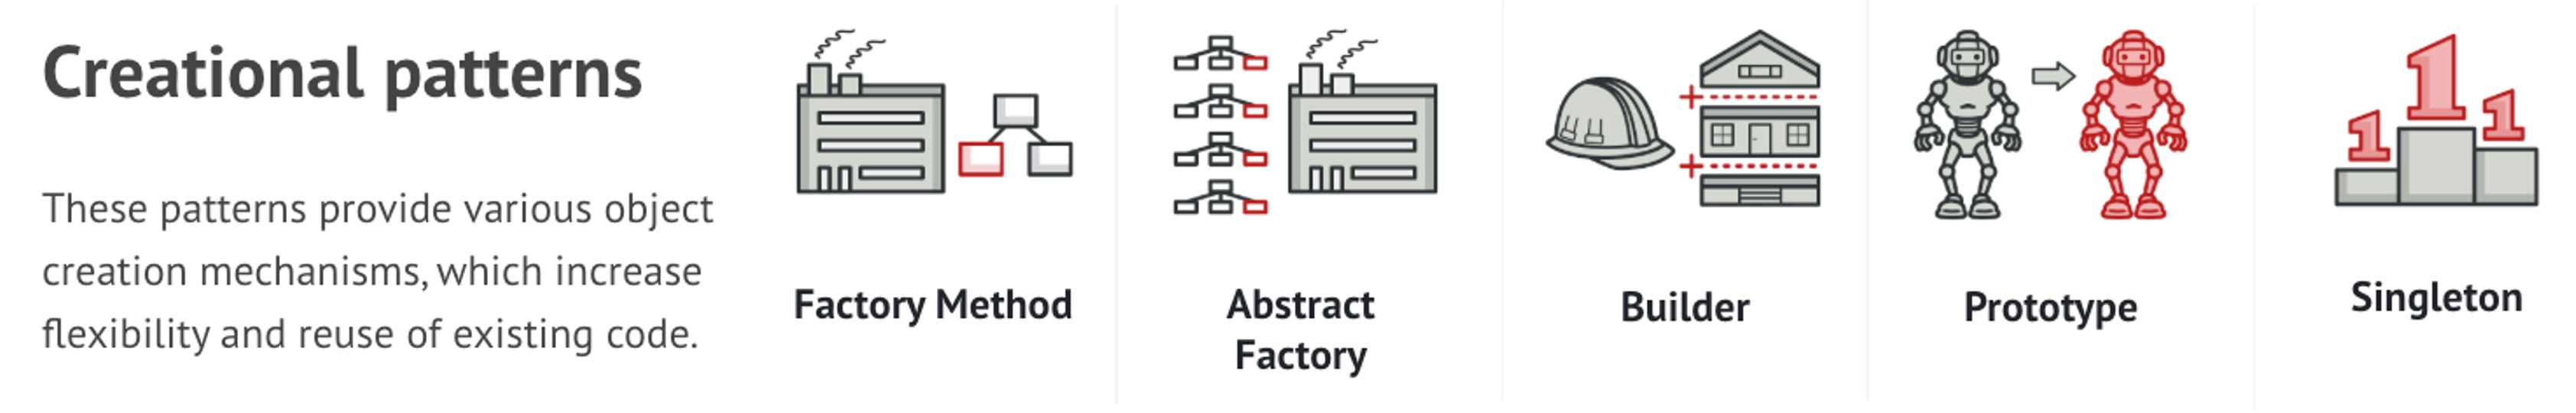
\includegraphics[width=1\linewidth]{creationalPatterns.jpg}}
\centerline{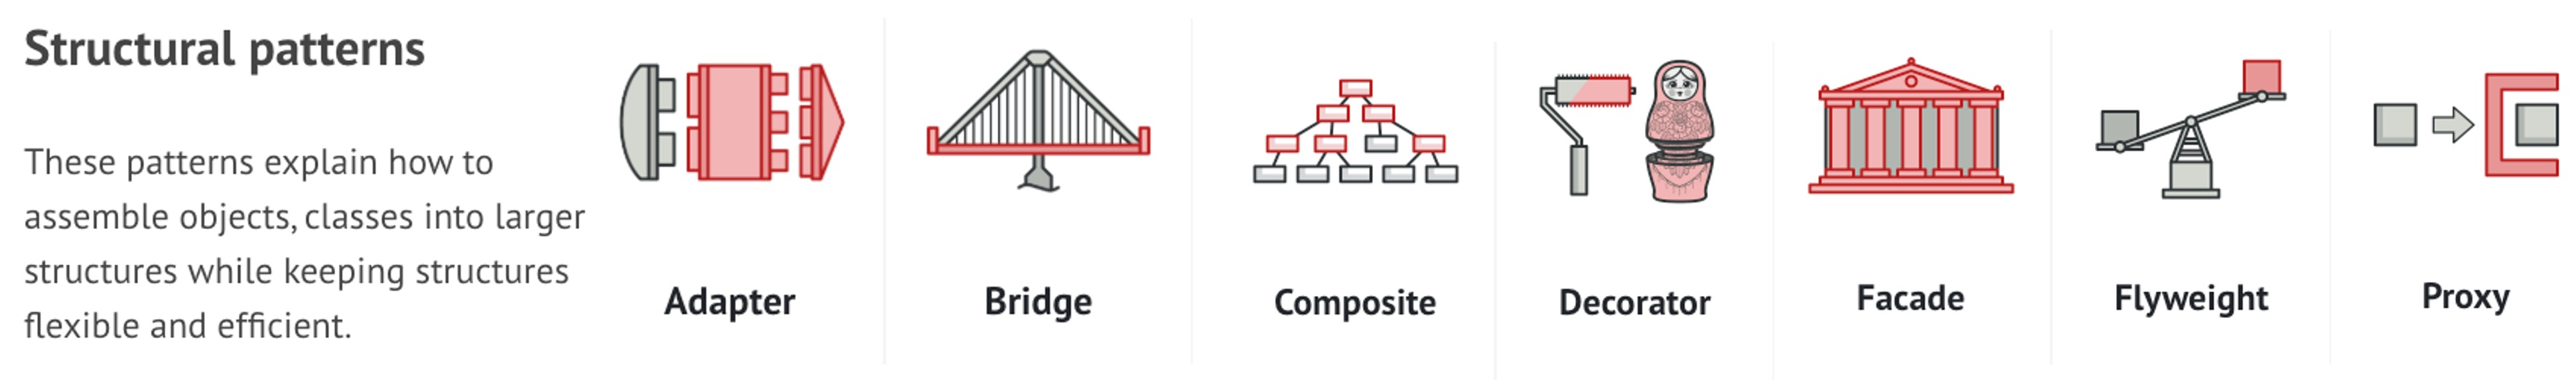
\includegraphics[width=1\linewidth]{structuralPatterns.jpg}}
\centerline{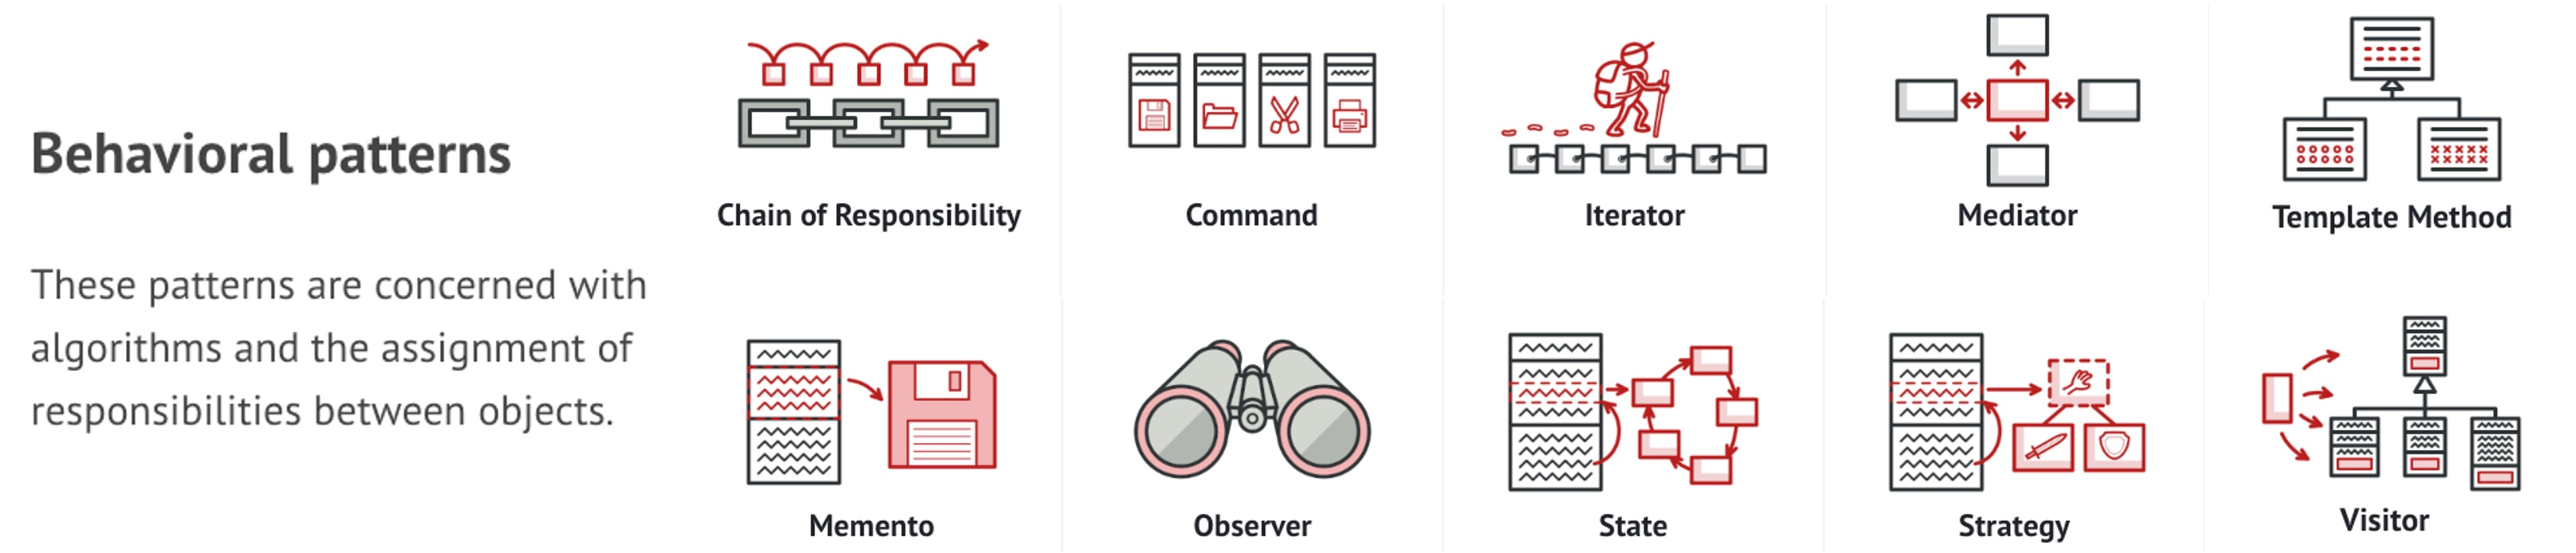
\includegraphics[width=1\linewidth]{behavioralPatterns.jpg}}

Read at https://refactoring.guru/design-patterns/catalog \href{https://refactoring.guru/design-patterns/catalog}{here}.

\null

\subsubsection{E.g. Factory Method}
Provides an interface for creating objects in a superclass, but allows subclasses to alter the type of objects that will be created. Suggests to replace direct object construction calls (using the \texttt{new} operator) with calls to a special factory method. 

\begin{itemize}
  \item Objects are still created via the \texttt{new} operator, but only inside the factory method. Objects returned by the factory method are often referred to as products.
  \item Then, override factory method in subclasses to change class of products created.
  \item Code that uses the factory method works with the resulting products through their base interface. This way, the code remains independent of the concrete product classes.
\end{itemize}

\null
\columnbreak

\subsection{Presentation Patterns (UI)}

Presentation patterns, often used in Mobile application, define how responsibilities are structured to improve maintainability, testability, scalability. E.g. MVC, MVP, MVVM.

\begin{itemize}
  \item Good architecture enforces separation of concerns, improves unit testability, reduces long-term maintenance cost, and prevents overly large UI components (e.g.\ Massive View Controllers).
  \item ELI5: Stop putting database code inside button click listeners etc.
\end{itemize}

\subsubsection{Scope within the System Architecture}

It is important to distinguish between \textit{Presentation Patterns} and \textit{System Architectures}.

\begin{itemize}
    \item \textbf{System Architecture (Macro Level)}: Patterns such as \textit{Layered Architecture}, \textit{Clean Architecture}, or \textit{Hexagonal Architecture} dictate the structure of the entire application (e.g., separating the Data Layer, Domain Layer, and Presentation Layer).
    \item \textbf{Presentation Pattern (Micro Level)}: Patterns like MVVM or MVC dictate the internal structure of the \textit{Presentation Layer} only.
\end{itemize}

A robust application typically utilizes both: a high-level System Architecture to organize the backend/data flow, and a Presentation Pattern to organize the UI components. E.g. a \textit{Clean Architecture} system,  outermost "Interface Layer" is structured internally using \textbf{MVVM}.

\subsubsection{MV(X) essentials: MVC, MVP, MVVM, VIPER}
\begin{itemize}
  \item \textbf{Overview}: All MV(X) patterns separate concerns into Model (domain data and business logic, which manipulates the data), View (UI rendering), and some intermediary component that mediates between Model and View. (Responsible for altering Model based on user input, updating View based on Model changes).
  \item Dividing entities allows for better understanding, reuse, and testability.
  \item \textbf{Model--View--Controller (MVC)}: MVC separates an application into Model (domain data and business logic), View (UI rendering), and Controller (mediate between Model and View). 
  \item \textbf{Usage:} Suitable for small applications, prototypes, or screens with limited logic where development speed is prioritised over testability. MVC traditionally used in iOS UIKit development, tho View Controllers become 'Massive VCs' due to accumulating too much responsibility.
  \item \textbf{Model--View--Presenter (MVP)}:MVP treats the view controller as a dumb passive View that forwards user events to a Presenter. The Presenter contains presentation logic and updates the View through an interface, with no direct View--Model dependency.
  \item Excellent testability, cost of increased boilerplate, manual binding between View, Presenter.
  \item \textbf{Model--View--ViewModel (MVVM)}:MVVM introduces a ViewModel that represents UI state independently of the UI framework. The View binds to observable properties exposed by the ViewModel, which updates the Model and reflects changes back to the View.
  \item MVVM improves testability, reduces UI update code because of binding mechanisms (e.g.\ LiveData, StateFlow, Rx). However, reactive flows can be harder to debug if poorly structured.
  \item \textbf{VIPER}: VIPER further decomposes responsibilities into View, Interactor (business and data logic), Presenter (UI logic), Entity (data models), and Router (navigation).
  \item Strongest separation of concerns and testability but significant boilerplate and maintenance overhead, making it suitable primarily for large or complex applications.
\end{itemize}

\subsection{Considerations and Choosing a Pattern}
% https://medium.com/ios-os-x-development/ios-architecture-patterns-ecba4c38de52#.rlbei1qau
\begin{itemize}
  \item \textbf{ELI5 Summary}: 
    \begin{itemize}
      \item \textbf{MVC}: (Triangle architecture) Controller, has routing logic, tells model what data to update, and view the flow (which view to use, navigation). View observes model directly and gets the data from model, exists coupling between view and model. (E.g. login screen click, controller tells model to fetch data, then selects which view to display).
      \item \textbf{MVP}: (Bridge architecture) Presenter sits strictly between View and Model. View is passive and dumb, presenter tells view what to do. View never observes model changes. (E.g. login screen, click a link, view tells presenter, presenter tells model to fetch data, uses data to tells view how to update). Separated, so easier unit testing.
      \item \textbf{MVVM}: (Reactive) ViewModel (Middleman) holds (UI state + UI logic), but never talks directly or holds reference to View (UI elements + rendering logic), sits there holding variables. View binds (observes) ViewModel variables, and updates reactively. Model also does not know ViewModel exists. 
      \item (E.g. login screen, click a link, view tells ViewModel, ViewModel tells model (business state + business logic) to fetch data, ViewModel (UI state) reacts to model changes, View (UI) auto-updates by observing ViewModel, and handles its own navigation of Views).
    \end{itemize}
   
  \item \textbf{Platform Considerations}: iOS (UIKit): MVC, MVVM, VIPER; iOS (SwiftUI): MVVM; 
  \item Android (XML / Compose): MVVM (recommended), MVP (legacy).
  \item \textbf{Overall}: No single best pattern. Simpler patterns favour dev speed, lower overhead, more structured ones improve testability and scalability at higher maintenance cost.
  \item Choose based on project constraints and team experience.
\end{itemize}


\section{Lecture B: Specification \& Abstraction}

\subsection{Software Development Processes}
\begin{itemize}
  \item \textbf{Waterfall Model}: A linear, sequential development process consisting of: Requirement Specification, Software Design \& Architecture, Implementation \& Integration, Testing \& Validation, Deployment \& Maintenance. Each phase must be completed before the next begins.
  \item \textbf{Spiral Model}: An iterative, risk-driven process with four main activities: Determine objectives \& constraints, Identify and resolve risks, Development and testing, Plan the next iteration. Emphasizes early risk mitigation.
  \item \textbf{Agile Model}: An iterative and incremental process emphasizing rapid feedback: Design, Build, Test, Release, Configure.
\end{itemize}

\subsection{Decomposition and Abstraction}
\begin{itemize}
  \item \textbf{Decomposition}: Breaking down a complex problem into smaller, manageable sub-problems. Each sub-problem is roughly at the same level of detail, can be solved independently, and can be combined to solve the original problem.
  \item \textbf{Abstraction}: Focusing on high-level specifications while hiding implementation details. Abstraction allows independence from specific implementations, enabling flexibility and easier maintenance.
\end{itemize}

\subsection{Abstraction}
\begin{itemize}
  \item \textbf{Abstraction by Parameterization}: Common computation patterns are abstracted using parameters. E.g. $x \times x + y \times y$ can be abstracted as: $\lambda x, y: x*x + y*y$. This allows reuse and generalization.
  \item \textbf{Abstraction by Specification (Contracts)}: Specifications as Contracts between client and implementer. Each procedure associated with specification defining how it can be used and what it guarantees. 
  \item If procedure A calls procedure B, A relies only on B's specification (locality), not its implementation. B can be reimplemented without affecting A (modifiability).
  \item This simplifies design, facilitates change, and improves maintainability. Complicated specifications often indicate poor design.
\end{itemize}

\subsection{Types of Abstraction}
\begin{itemize}
  \item \textbf{Procedural Abstraction}: Abstracting common computation patterns into procedures with well-defined specifications. Abstracts implementation from intent, should be minimalist (few constraints on usage), underdetermined (allow multiple implementations), deterministic (same input produces same output), and general (handles wide class of inputs).
  \item Total procedures defined for all legal inputs, partial procedures undefined for some inputs (must include REQUIRES clause). Procedure specifications include REQUIRES (conditions assumed true), RETURNS, MODIFIES, and EFFECTS.
  \item \textbf{Data Abstraction}: Abstract Data Types (ADTs) encapsulate data representation and operations. Data can only be accessed through its operations, improving maintainability and allowing representation changes for efficiency.
  \item An abstraction function maps concrete state to abstract state, while a representation invariant is a predicate that must always hold for the concrete representation. A \texttt{checkRep} function verifies the representation invariant. Rep invariant should be first thing articulated, not an afterthought.
  \item \textbf{Iteration Abstraction}: Instead of exposing internal structure, provide a way to iterate over elements. This allows changing the underlying representation without affecting clients.
  \item Iteration can be implemented in several ways: returning all elements at once (arrays), storing traversal state inside collection itself, using external iterator objects, or using closures. Must consider simplicity, efficiency, and control. Iterator-based approaches must handle tracking the current position, avoid duplicated work between hasNext and next, and ensure correctness when the underlying collection is modified, often by invalidating the iterator.
  \item \textbf{Type Hierarchy}: Organizing types into a hierarchy based on shared characteristics. Subtyping allows substituting objects of a subtype for those of a supertype, preserving behavior. This enables polymorphism and code reuse.
  \item \textbf{Polymorphic Abstraction}: Allows code to work over many types. Approaches include using type hierarchies (subtyping) or requiring only necessary operations (structural typing). Example: A sorting function that works for any type that supports comparison, even if the types are unrelated.
\end{itemize}

\columnbreak
\section{Lecture 3: Memory Management \& Initialisation}

Two related pillars of Swift's safety model:
\textbf{safe initialisation} and \textbf{automatic memory management}. Swift enforces many rules at compile time to prevent undefined behaviour such as using uninitialised memory or accessing deallocated objects. Understanding these rules is essential for writing correct, crash-free applications.

\subsection{Initialisation}

Initialisation in Swift is deliberately strict. Unlike some languages that allow partially initialised objects, Swift requires that all stored properties have well-defined values before they are used. This design eliminates an entire class of runtime errors.

\subsubsection{Swift Variables}
Swift enforces \textbf{definite initialisation}, where every variable must be initialised before it is read, and the compiler checks \emph{all possible execution paths}.

There are no implicit default values for variables, except for optionals which default to \texttt{nil}.

\begin{verbatim}
var message: String
if lectureStarted {
  message = "You should be taking notes."
}
print(message) // ERROR: variable 'message' used before initialized
\end{verbatim}

Even of \texttt{message} may be initialised at runtime, compiler rejects code as there exists a path where it is not.

\subsection{Initialisers}

Initialisers are special methods whose sole responsibility is to put an instance into a valid, usable state. Swift treats initialisation as a safety-critical phase and restricts what code can do during it.

\begin{itemize}
  \item Initializing applies to \texttt{struct}, \texttt{enum}, and \texttt{class}
  \item All stored properties must be initialised exactly once, and before use
  \item \textbf{What Does ``Before Use'' Mean}: \texttt{self} cannot be accessed, instance methods cannot be called, properties cannot be read before initialisation is complete.
  \item This prevents code from observing or operating on a partially initialised object.
\end{itemize}

\subsection{Safe Initialisation}

\begin{verbatim}
struct Color {
  var red: Int, green: Int, blue: Int

  init(red: Int, green: Int, blue: Int) {
    self.red = red
    self.green = green
    self.checkRep() // ERROR: self used before... initialized
    self.blue = blue
  }

  func checkRep() {
    assert(red > 0 && green > 0 && blue > 0)
  }
}
\end{verbatim}

Calling methods before all stored properties are initialised is forbidden. Even though \texttt{checkRep} looks harmless, it implicitly accesses \texttt{self}.

\subsection{Initialising Classes}

Class initialisation is more complex due to inheritance. Swift enforces strict ordering to ensure subclasses cannot observe uninitialised superclass state (and vice versa).

\subsubsection{Subclass Initialisation Order}

\begin{verbatim}
class Car {
  var paintColor: Color
  init(color: Color) {paintColor = color}
}

class RaceCar: Car {
  var hasTurbo: Bool
  init(color: Color, turbo: Bool) {
    super.init(color: color) // ERROR: 'hasTurbo' not initialized
    hasTurbo = turbo
  }
}
\end{verbatim}

\textbf{Rule:} A subclass must initialise all of its own stored properties \emph{before} calling \texttt{super.init}.

\subsubsection{Calling Methods During Initialisation}

Calling instance methods during initialisation is dangerous bc. subclasses may override them.

\begin{verbatim}
class Car {
  init(color: Color) {
    paintColor = color
    fillGasTank()
  }
}
\end{verbatim}

If \texttt{fillGasTank} is overridden, it may execute before subclass properties are initialised.

\subsection{Overloading Initialisers}

Swift distinguishes between two kinds of initialisers to control complexity and ensure safety.

\subsubsection{Designated vs Convenience Initialisers}

\begin{itemize}
  \item \textbf{Designated Initialisers}: Primary inits, fully initialises all properties introduced by class
  \item \textbf{Convenience Initialisers}: Secondary, helper inits, provide defaults or alternative parameter lists (syntax: \texttt{convenience init(params)} $\{ ... \}$)
  \item \textbf{Initializer Delegation Rules}: Strict delegation hierarchy:
    \begin{itemize}
      \item Designated initialisers must call a designated initialiser of the immediate superclass
      \item Convenience initialisers must call another initialiser in the same class
      \item Convenience initialisers must eventually call a designated initialiser
    \end{itemize}
  \item \textbf{Safety Checks}: All properties introduced by class must be init before delegating to super class. Designated inits must delegate to superclass before modifying any inherited property.
  \item A convenience init must delegate to another init before it assigns any property. Initializer cannot call any instance method, read property values, or refer to \texttt{self} before delegating.
\end{itemize}

\subsection{Two-Phase Initialisation}

Swift class init happens in two distinct phases to guarantee safety across inheritance chains.

\begin{itemize}
    \item \textbf{Phase 1}: Each class initialises the properties it introduced. Memory becomes fully allocated
    \item \textbf{Phase 2}: Each class can further customise the instance (e.g. call methods, modify properties). Instance is fully valid.
\end{itemize}


\subsection{Initializer Inheritance}

Initialisers are not inherited by default. This prevents subclasses from accidentally exposing unsafe or incomplete initialisation paths.

\begin{itemize}
  \item \textbf{Automatic Initializer Inheritance}: Automatic inheritance occurs only when Swift can prove it is safe. 
  \item If subclass does not define any designated initialisers, it automatically inherits all of its superclass's designated initialisers.
  \item If subclass overrides all superclass designated initialisers, it automatically inherits all of the superclass's convenience initialisers.
\end{itemize}

\subsection{Memory Management}

Swift abstracts away manual memory management while still providing deterministic performance characteristics.

\subsubsection{Stack vs Heap}

\begin{itemize}
  \item \textbf{Stack}: fast, automatic, limited lifetime
  \item \textbf{Heap}: flexible size, managed via reference counting
  \item Objects and closures live on the heap.
\end{itemize}

\subsection{Manual Retain Release (MRR), Automatic Reference Counting (ARC)}

\begin{itemize}
  \item \textbf{Manual Retain Release}: Before ARC, Objective-C required programmers to manually manage ownership: \texttt{retain} to claim ownership, \texttt{release} to relinquish ownership. This was powerful but extremely error-prone.
  \item \textbf{Auto Reference Count}: ARC automates reference counting at compile time. ARC inserts retain/release calls automatically based on variable scope and assignments. Objects deallocate immediately when reference count hits zero.
  \item This gives Swift deterministic deinitialisation without runtime pauses. ARC allows us to write code naturally, not worry and concentrate on app. - ARC is not garbage collection, as it is deterministic and does not require pauses.
  \item \textbf{Garbage Collection}: Commonly refers to Mark and Sweep algorithm, periodically pauses execution to reclaim unreachable memory. (Used in Java, Python, Ruby). Mark live objects from root, sweep heap to free unmarked objects, no need to worry about cycles.
  \item GC (vs. ARC) requires 2-3 times more memory (android phones need more RAM), suspends execution during collection, unpredictable performance, but ease on programmer. 
  \item ARC (vs. GC) has less memory overhead, deallocation compiled into program, deterministic deinitialisation, but programmer must manage reference cycles and leaks.
\end{itemize}

\subsection{Swift Reference Types}
Classes and closures are reference types in Swift. Variables store references (pointers) to heap-allocated objects.

\begin{itemize}
  \item \textbf{Strong References}: Default in Swift, increase reference count
  \item \textbf{Weak References}: Do not increase reference count, must be optional type as becomes nil if object is deallocated.
  \item \textbf{Unowned References}: Do not increase reference count, non-optional. Assume referenced object always exists during lifetime of reference.
\end{itemize}

\centerline{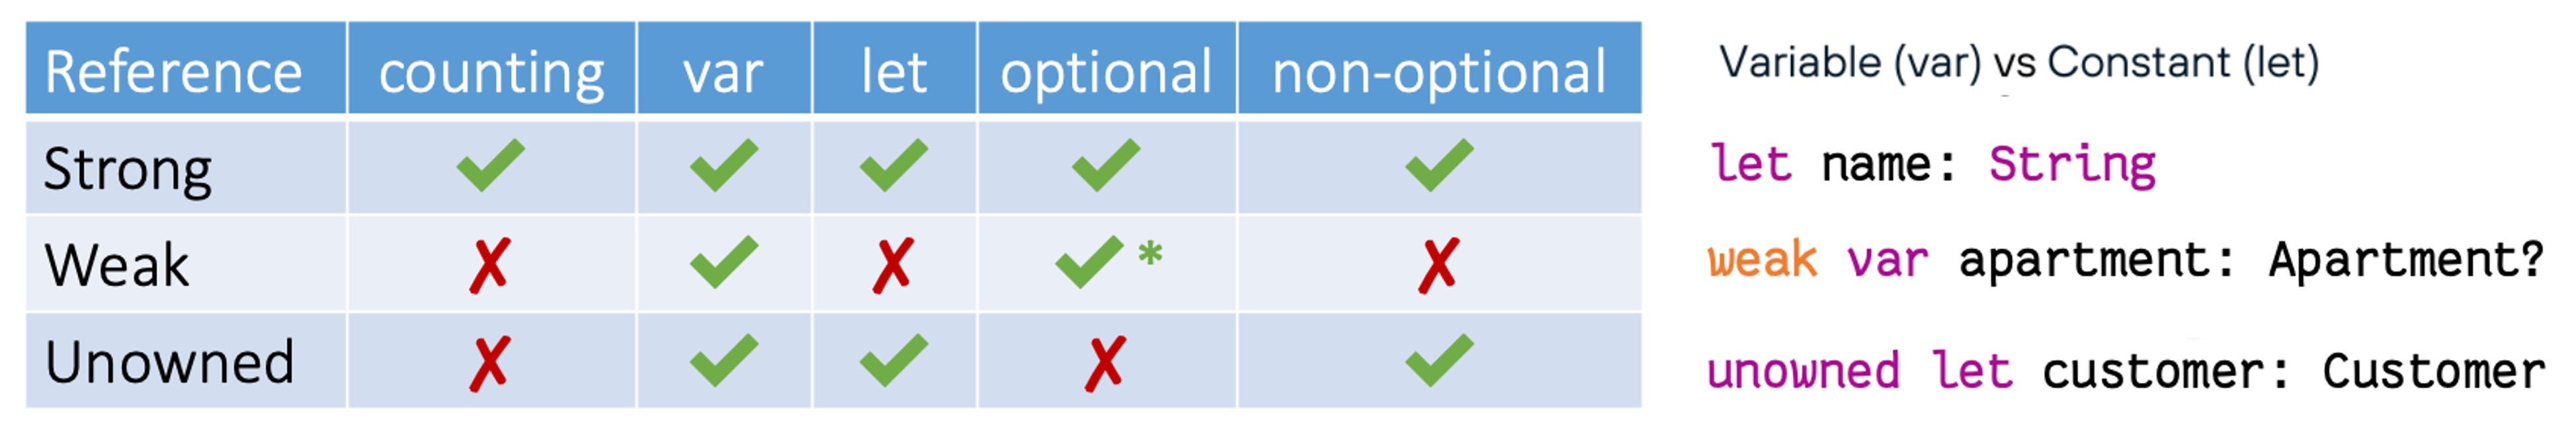
\includegraphics[width=0.85\linewidth]{referenceTypes.jpg}}

\subsection{Reference Counting and Cycles}
\begin{itemize}
  \item \textbf{Reference Counting}: Each object has a reference count tracking how many strong references point to it. When reference count reaches zero, object is deallocated.
  \item \textbf{Strong Reference Cycles}: ARC cannot break cycles automatically. If two objects strongly reference each other, their reference counts never reach zero. This results in memory leaks.
  \item \textbf{Weak and Unowned References}: Swift provides two tools to break reference cycles. Weak References do not increase reference count, must be optional and auto set to \texttt{nil} if object deallocated. Unowned References also do not increase reference count, but are non-optional and assume referenced object always exists.
\end{itemize}


\subsection{Choosing the Right Reference}
\begin{itemize}
    \item \textbf{strong} references $\rightarrow$ use for owners to objects they own.
    \item Both sides (properties) can be nil, optional $\rightarrow$ use \textbf{weak}. Use among objects with independent lifetimes.
    \item One side optional $\rightarrow$ use \textbf{unowned}. Use from owned objects with same lifetime.
    \item Neither optional $\rightarrow$  use \textbf{implicitly unwrapped optional}
    \item \textbf{Implicitly unwrapped optional}: use when property cannot be initialised immediately but is guaranteed to exist after initialisation. (E.g. \texttt{var capital: City!}). Behaves like non-optional after initialisation but allows deferred setup.
\end{itemize}

\subsection{Closures and Reference Cycles}

Closures are reference types and capture variables strongly by default.
\begin{itemize}
  \item \textbf{Closures}: are reference types that capture variables strongly from their surrounding context.
  \item Common source of memory leaks, especially when stored as properties
  \item \textbf{Capture Lists}: used to control how values are captured (strong, weak, unowned)
  \begin{verbatim}
  lazy var closure = { [unowned self] in
    self.doSomething()
  }
  \end{verbatim}
\end{itemize}

\subsection{Reference Cycles in Structs}

Although structs are value types, they can still participate in reference cycles if they store reference types.

\begin{itemize}
    \item Cycles occur indirectly via heap-allocated objects
    \item Swift currently provides no direct mechanism to break them
\end{itemize}

This highlights that ARC issues are about \emph{references}, not value semantics alone.

\columnbreak

\section{Lecture C: Value Type Semantics}

Swift design philosophies: \textbf{value type semantics}. Use of value type encouraged to reduce bugs caused by unintended sharing, improve reasoning about code, and enable safer concurrency. Contrast value semantics with reference semantics, examine common pitfalls, and study how Swift achieves efficiency through copy-on-write.

Swift's model combines mutability where needed, with value semantics (immutability) by default and efficiency through copy-on-write.

Understanding how to mix value and reference types correctly is key to writing robust Swift programs.

\subsection{Reference Semantics vs Value Semantics}

At a high level, understanding the distinction is crucial when designing APIs and data models.
\begin{itemize}
  \item \textbf{Reference semantics}: multiple variables can refer to the same instance
  \item \textbf{Value semantics}: each variable has its own logically independent copy
\end{itemize}


\subsection{Reference Semantics}
Reference types (classes) allow shared mutable state. While powerful, this can lead to subtle bugs when changes in one place affect another unexpectedly.

\subsubsection{Example: Temperature Class}

\begin{verbatim}
class Temperature {
    var celsius: Double = 0
    var fahrenheit: Double {
        get { return celsius * 9 / 5 + 32 }
        set { celsius = (newValue - 32) * 5 / 9 }
    }
}

let temp = Temperature()
temp.celsius = 24
home.thermostat.temperature = temp

temp.celsius = 180
home.oven.temperature = temp
\end{verbatim}

Classes are reference types, meaning assignments copy the reference, not the value. Both the thermostat and oven now point to the same \texttt{Temperature} instance. Mutating \texttt{temp} affects both — often unintentionally.

\subsection{Copying as a Fix (and Its Problems)}

One way to avoid unintended sharing is copying, but this approach scales poorly.
\begin{itemize}
  \item \textbf{Manual Copying}: Programmer must remember to copy objects whenever sharing is undesirable. This relies on discipline and is error-prone.
  \begin{verbatim}
  home.thermostat.temperature = temp.copy()
  home.oven.temperature = temp.copy()
  \end{verbatim}
  \item \textbf{Defensive Copying}: Classes defensively copy inputs in setters. Every setter must defensively copy. This pattern is tedious, error-prone, and does not compose well.
  \begin{verbatim}
  var temperature: Temperature {
      get { return _temp }
      set { _temp = newValue.copy() }
  }
  \end{verbatim}
  \item \textbf{Framework-Level Copying}: Some frameworks (e.g. Objective C, Cocoa Touch) enforce copying via protocols or property attributes. Howeverm missed copies can still cause bugs.
\end{itemize}

\subsection{Immutability}

Immutability reduces bugs by preventing mutation altogether.
\begin{itemize}
  \item \textbf{Example}: Make \texttt{Temperature} immutable by declaring properties as \texttt{let} and removing setters.
  \begin{verbatim}
  class Temperature {
      let celsius: Double
      var fahrenheit: Double { celsius * 9 / 5 + 32 }
  }
  \end{verbatim}
  \item Now, once created, \texttt{Temperature} instances cannot be modified. This eliminates unintended sharing issues.
  \item While safer, immutable reference types can lead to awkward APIs that require creating new objects for small changes.
  \item \textbf{Immutability vs Performance}: Immutable data structures can have worse asymptotic performance:
    \begin{itemize}
        \item Mutable algorithms: $O(n)$
        \item Immutable rebuilding: $O(n^2)$
    \end{itemize}
\end{itemize}



\subsection{Value Semantics}

Swift aims to balance safety and performance. Value semantics provide:
\begin{itemize}
    \item Independent copies by default, Local reasoning about mutations and hence fewer unintended side effects
    \item \textbf{Logically distinct variables}: E.g. \texttt{var a = 17; var b = a; b += 25} means \texttt{a} remains 17, \texttt{b} becomes 42. Mutating \texttt{b} does not affect \texttt{a}.
    \item This behavior extends to user-defined types (structs, enums), strings, arrays, sets, and dictionaries.
\end{itemize}

\subsection{Value Types in Swift}

All fundamental Swift types are value types:
\begin{itemize}
    \item Scalars: \texttt{Int}, \texttt{Double}, \texttt{Bool}
    \item Collections: \texttt{Array}, \texttt{Set}, \texttt{Dictionary}, \texttt{String}
    \item Custom types: \texttt{struct}, \texttt{enum}, tuples
\end{itemize}

\subsection{Equality, Equatable Value Types}

\begin{itemize}
  \item Value types are compared by \textbf{value}, not identity. (E.g. \texttt{==} compares contents, not memory addresses, so two distinct strings with the same characters are considered equal).
  \item \textbf{Equatable}: Value types should conform to \texttt{Equatable}. This allows using \texttt{==} to compare instances based on their values.
  \begin{verbatim}
  struct Point {
    var x: Float
    var y: Float
  }

  extension Point: Equatable {
    static func ==(lhs: Point, rhs: Point) -> Bool {
      lhs.x == rhs.x && lhs.y == rhs.y
    }
  }
  \end{verbatim}
  \item \textbf{Example}: Value-Type Temperature. Rewriting \texttt{Temperature} as a struct allows each assignment to create an independent copy, eliminating unintended sharing.
  \begin{verbatim}
  struct Temperature {
    var celsius: Double = 0
    var fahrenheit: Double {
      get { celsius * 9 / 5 + 32 }
      set { celsius = (newValue - 32) * 5 / 9 }
    }
  }
  \end{verbatim}
  \item \textbf{Equatable with Reference type properties}: If a value type contains reference type properties, equality must be defined carefully to ensure logical equivalence. Identity comparison (\texttt{===}) is insufficient. Use deep equality to compare the contents of referenced objects. (E.g. \texttt{lhs.image.isEqual(rhs.image)}).
\end{itemize}

\subsection{Let vs Var for Value Types}

\begin{itemize}
    \item \texttt{let} value type: cannot mutate any property
    \item \texttt{var} value type: mutation allowed
\end{itemize}

This enforces immutability at the variable level, not just the property level.

\subsection{Value Semantics Benefits and Performance}

\begin{itemize}
    \item \textbf{Benefits}: Freedom from race conditions,sSafe mutation during iteration and easier reasoning in concurrent code.
    \item \textbf{Performance}: Copies are kept cheap via optimizations like copy-on-write. Small value types take constant time, large collections and data structures are copy on write. (Actual copy deferred until mutation).
\end{itemize}


\subsection{Mixing Value and Reference Types}
Mixing value and reference types can lead to unexpected behavior if not done carefully.

\begin{itemize}
  \item \textbf{Reference in Value type}: If a value type contains a reference type property, copies of the value type will share the same reference. Mutating the referenced object affects all copies. Violates intuitive value semantics.
  \item \textbf{Value in Reference type}: If a reference type contains value type properties, each instance gets its own copy of the value-type properties. This generally preserves expected behavior.
  \item \textbf{Mutable References inside Value type}: If a value type contains mutable reference type properties, mutations to the referenced object affect all copies of the value type. This can lead to unexpected shared mutation.
  \item Use copy on write pattern to ensure mutations happen on private copies only.
\end{itemize}

\subsection{When to Use Value types vs Reference types}

Reference semantics enable sharing but risk unintended mutation.  
Value semantics provide safer defaults, better composability, and easier concurrency.  

\textbf{Use value types when:}
\begin{itemize}
    \item Equality matters more than identity
    \item Copies should be independent
    \item Data crosses thread boundaries
\end{itemize}

\textbf{Use reference types when:}
\begin{itemize}
    \item Identity matters
    \item Shared mutable state is intentional
\end{itemize}

\null \null

\section{Tutorial 1: Data Structures, Error Handling, Language Design}

\subsection{Efficient Data Structures}

\begin{itemize}
    \item Choosing the right implementation matters: e.g., arrays vs linked lists for stacks and queues affect time complexity.
    \item Invariants and representation checks are crucial for correctness.
    \item Design decisions should balance performance, memory usage, and simplicity.
\end{itemize}

\subsection{Abstract Data Type (ADT) Design}

\begin{itemize}
    \item Graphs and trees can be implemented with different representations depending on expected use cases (sparse vs dense, generality vs simplicity).
    \item Reusing existing ADTs can save effort, but sometimes a specialized implementation is clearer.
    \item Test-driven development ensures each operation meets specifications, guides cleaner design.
\end{itemize}

\subsection{Error Handling Principles}

\begin{itemize}
    \item Different ways to handle errors: return special values, use optionals (nullable types), or throw exceptions.
    \item Choose a strategy based on whether errors are expected, recoverable, or exceptional.
    \item Explicit handling improves safety and maintainability; silent failures may lead to bugs.
\end{itemize}

\subsection{Code Readability and Comments}

\begin{itemize}
    \item Comments should clarify \textbf{why} something is done, not \textbf{what} the code literally does.
    \item Redundant comments add noise and reduce readability.
    \item Clear code often reduces the need for explanatory comments.
\end{itemize}

\subsection{Type Conversion and Language Design Choices}

\begin{itemize}
    \item Different languages handle type conversion differently, reflecting their design philosophy (safety vs convenience).
    \item Safe conversions (e.g., optional types, exceptions) encourage explicit handling of invalid input.
    \item When designing APIs or structs, favor approaches that make failure explicit to the caller, improving robustness.
\end{itemize}

\subsection{Key Takeaways}

\begin{itemize}
    \item Focus on abstraction and correctness before optimization.
    \item Explicit error handling and careful ADT design improve code safety and maintainability.
    \item Immutability, clear invariants, and value vs reference semantics support safer concurrent and modular code.
    \item Write tests to guide implementation and verify correctness.
\end{itemize}

\columnbreak 


\section{Tutorial 2: TDD, Functional and Imperative Paradigms}
\subsection{Test-Driven Development (TDD) and ADTs}

\begin{itemize}
    \item Define tests before implementing functionality; guides API design and ensures correctness.
    \item Consider edge cases, invalid input, and expected behaviors when designing tests.
    \item For game or domain ADTs (e.g., Tic-Tac-Toe), tests should cover state transitions, win/loss conditions, and invalid moves.
    \item TDD encourages modular and testable code.
\end{itemize}

\subsection{Test Doubles and Dependency Injection}

\begin{itemize}
    \item \textbf{Test doubles} (mocks, stubs, fakes) simulate external dependencies to isolate unit under test.
    \item \textbf{Dependency injection} allows passing dependencies (e.g., databases, services) into components, making testing easier.
    \item Useful when external systems are slow, non-deterministic, or hard to set up.
    \item Less useful when dependencies are simple, stable, or tightly coupled to internal logic.
\end{itemize}

\subsection{Single Level of Abstraction Principle (SLAP)}

\begin{itemize}
    \item Functions should operate at a single level of abstraction.
    \item Mixing details and high-level logic in a function makes code harder to read, test, maintain.
    \item Refactor long, complex functions into small, focused helper functions improves clarity, reuse.
\end{itemize}

\subsection{Delegate Pattern and UI Design}

\begin{itemize}
    \item Delegates allow separation of concerns: UI components handle display, while domain logic is handled externally.
    \item Delegates are defined via protocols/interfaces specifying methods that UI component can call.
    \item Improves modularity, testability, and reusability of UI components.
    \item Example: A grid view component delegates user input handling to a separate class.
\end{itemize}

\subsection{Functional Core, Imperative Shell Paradigm}
\begin{itemize}
  \item \textbf{Pattern}: Having a functional core where all pure functions (no side effects, immutable) live, and thin imperative shell where impure functions operate.
  \begin{itemize}
    \item Core logic is \textbf{purely functional}: deterministic, no side effects, easy to reason about, test.
    \item Shell handles \textbf{imperative concerns}: I/O, state mutation, user interaction, interact with outside world; usually thin and minimally tested.
  \end{itemize}
  \item \textbf{Advantages of Functional Core, Imperative Shell}: Easier testing: functional core extensive tests. Predictable behavior and fewer bugs. Clear separation of pure logic and side effects.
  \item \textbf{Limitations}: Not always applicable for highly interactive or stateful systems where pure functional abstraction is difficult. Requires discipline to keep side effects confined to the shell.
  \item Related patterns: IO monad, Actor model, Flux/Redux architecture.
  \item \textbf{IO Monad (Functional Programming)}  
  \begin{itemize}
    \item Encapsulates side effects (e.g., file I/O, network calls) in a controlled, composable way.
    \item \textbf{ELI5}: Wrap effects in a function or container instead of performing them immediately. Basically, it is e.g. separating out parts of code that have side effects in a function, but still calling it all together when needed in a function.
    \item This lets you test the functional parts of the code for testing and makes it easier to reason and more predictable.
    \item Keeps the main program logic pure, deferr all effectful computations to a controlled context.
    \item Ensures predictability, easier testing, and reasoning about program behavior.
  \end{itemize}

  \item \textbf{Actor Model (Concurrent Systems)}  
  \begin{itemize}
    \item Everything is an actor, has independent private state, behavior, mailbox for message passing.
    \item State mutations confined to actors, resembling "imperative shell" around a functional core that processes messages.
    \item Promotes safe concurrency (actors no shared mutable state), encapsulation, scalability.
  \end{itemize}

  \item \textbf{Flux / Redux Architecture (Frontend State Management)}  
  \begin{itemize}
    \item Application state is immutable and updated by pure reducer functions (the functional core).
    \item Have Store, Reducer, Action, Dispatcher, View UI. Reducers are the functional core, UI components, middleware, API calls form the imperative shell, all handled outside reducers.
    \item Ensures predictable state transitions and simplifies testing, as the core logic is pure.
    \item Originated in the React ecosystem, but is an architecture pattern for predictable state management.
  \end{itemize}
\end{itemize}

\centerline{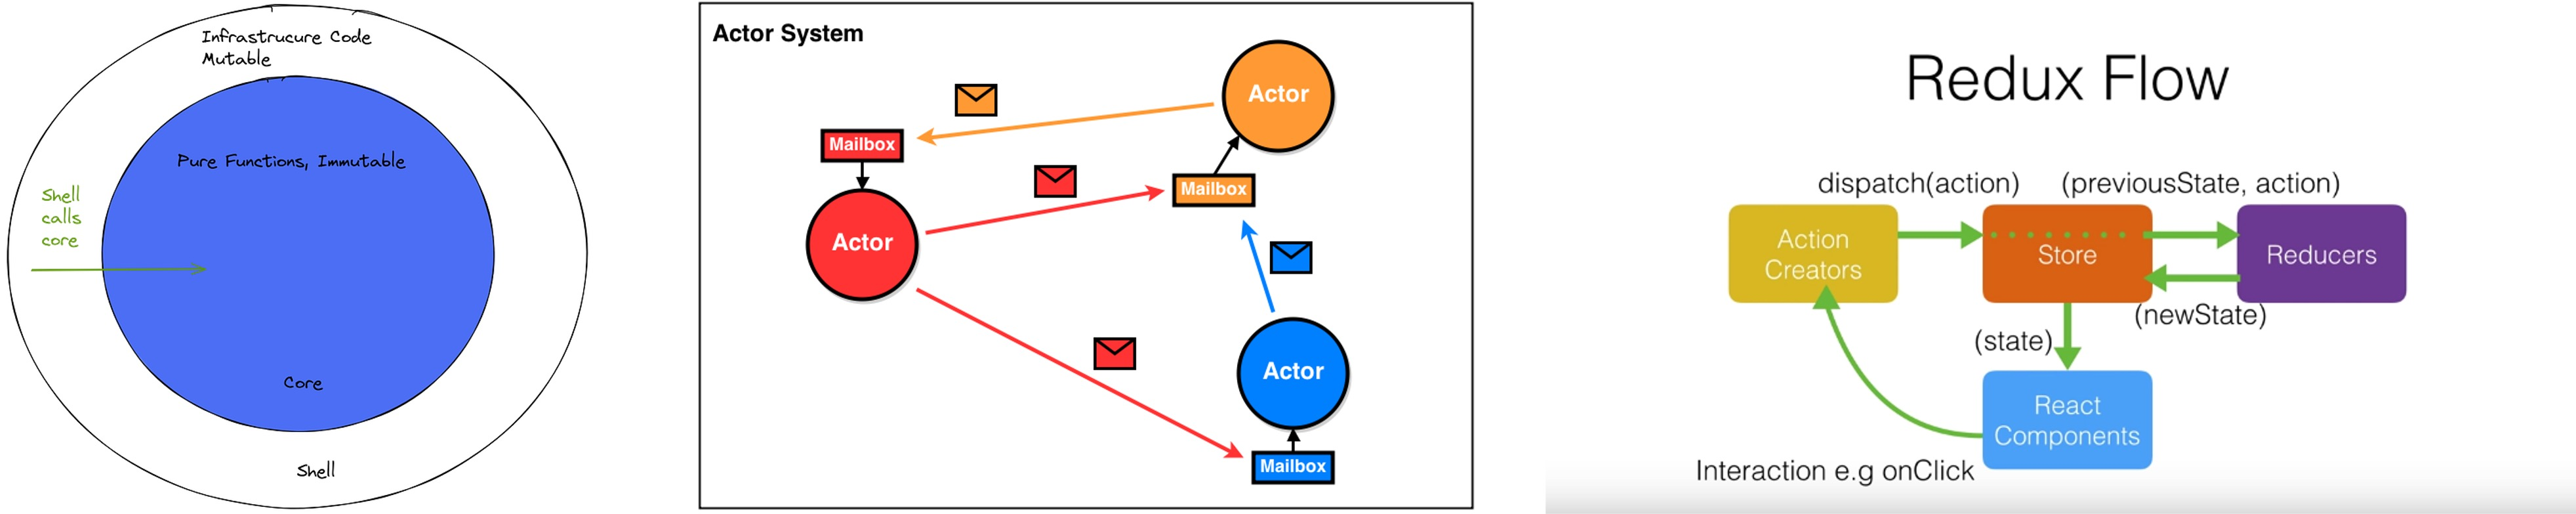
\includegraphics[width=\linewidth]{functionalCore.jpg}}


\section{Lecture 3.1: Objects and Data Structures}

\subsection{Data Abstraction}
\begin{itemize}
  \item \textbf{Goal}: hide representation and force clients to interact through meaningful operations.
  \item \textbf{Bad abstraction (data exposure)}: A \texttt{struct} with public fields exposes implementation, lets clients mutate fields independently, and makes invariants hard to enforce.
  \item \textbf{Better abstraction (protocol interface)}: Specify behavior in terms of operations, e.g. \texttt{setCartesian} and \texttt{setPolar} so coordinates are assigned consistently, and the representation (rectangular vs polar) can change.
\end{itemize}

\begin{verbatim}
struct Point {
  public var x = 0.0
  public var y = 0.0
}

protocol Point {
  var x: Double { get }
  var y: Double { get }
  mutating func setCartesian(x: Double, y: Double)
  var r: Double { get }
  var theta: Double { get }
  mutating func setPolar(r: Double, theta: Double)
}
\end{verbatim}

\begin{itemize}
  \item \textbf{Express in abstract terms}: prefer properties that state intent, not storage.
  \item E.g.: \texttt{percentOfFuelRemaining} hides tank size, internal units, can compute or cache.
\end{itemize}

\begin{verbatim}
protocol Vehicle {
  var fuelTankCapacityInGallons: Double { get }
  var gallonsOfFuel: Double { get }
}

protocol Vehicle {
  var percentOfFuelRemaining: Double { get }
}
\end{verbatim}

\subsection{Data/Object Anti-Symmetry}
\begin{itemize}
  \item \textbf{Objects}: hide data behind abstractions, expose functions that operate on that data.
  \item \textbf{Data structures}: expose data, have little to no behavior.
  \item These are complementary; mixing them blurs boundaries and weakens both.
\end{itemize}

\subsubsection{Procedural vs Object-Oriented}
\begin{itemize}
  \item \textbf{Procedural (data + functions elsewhere)}: easy to add new functions, but hard to add new data types (must update all functions).
  \item \textbf{Object-oriented (behavior with data)}: easy to add new types, but hard to add new functions (must update all classes).
  \item ``Everything is an object'' is a myth; pick the style based on expected change.
\end{itemize}

\begin{verbatim}
// Procedural
struct Square { var topLeft: Point; var side: Double }
struct Rectangle { var topLeft: Point; var height: Double; 
                    var width: Double }
struct Circle { var center: Point; var radius: Double }

struct Geometry {
  static let PI = 3.141592653589793
  func area(shape: Shape) throws {
    switch shape {
      case let s as Square: return pow(s.side, 2)
      case let r as Rectangle: return r.height * r.width
      case let c as Circle: return PI * pow(c.radius, 2)
      default: throw NoSuchShapeError
    }
  }
}

// Each time we add a new shape, we must update area()

\end{verbatim}

\columnbreak

\begin{verbatim}
// Object-Oriented
protocol Shape { var area: Double { get } }

struct Square: Shape {
  var topLeft: Point; var side: Double
  var area: Double { return pow(side, 2) }
}
struct Rectangle: Shape {
  var topLeft: Point; var height: Double; var width: Double
  var area: Double { return height * width }
}
struct Circle: Shape {
  static let PI = 3.141592653589793
  var center: Point; var radius: Double
  var area: Double { return PI * pow(radius, 2) }
}
// Each shape knows how to compute its own area
\end{verbatim}

\subsection{Law of Demeter (LoD)}
\begin{itemize}
  \item \textbf{Principle}: a module should not know the internals of the objects it manipulates.
  \item A method \texttt{f} of class \texttt{C} should only call methods of:
  \begin{itemize}
    \item \texttt{C} itself
    \item objects created by \texttt{f}
    \item objects passed as arguments to \texttt{f}
    \item objects held in instance variables of \texttt{C}
  \end{itemize}
\end{itemize}

\subsubsection{Train Wrecks}
\begin{verbatim}
String outputDir = sctxt.getOptions().getScratchDir().getAbsolutePath();
\end{verbatim}

\begin{itemize}
  \item Long chains expose internal structure (many coupled train cars).
  \item Splitting can improve readability but not necessarily LoD compliance.
\end{itemize}

\begin{verbatim}
Options opts = ctxt.getOptions();
File scratchDir = opts.getScratchDir();
String outputDir = scratchDir.getAbsolutePath();
\end{verbatim}

\begin{itemize}
  \item Whether this violates LoD depends on what \texttt{ctxt}, \texttt{Options}, \texttt{File} are.
  \item If they are objects, asking for internals violates LoD. If they are pure data structures, LoD does not apply.
\end{itemize}

\subsubsection{Hiding Structure vs Exploding APIs}
\begin{itemize}
  \item \texttt{ctxt.getAbsolutePathOfScratchDirectoryOption()} hides internals but can lead to method explosion.
  \item \texttt{ctxt.getScratchDirectoryOption().getAbsolutePath()} assumes returned value is a data structure.
  \item If \texttt{ctxt} is an object, we should \textbf{tell} it what we want done.
\end{itemize}

\subsubsection{Single Level of Abstraction}
\begin{itemize}
  \item The code below mixes multiple levels: string paths, separators, file extensions, and I/O streams.
  \item This is hard to read and easy to break if details change.
\end{itemize}

\begin{verbatim}
String outFile = outputDir + "/" + className.replace('.', '/')
  + ".class";
FileOutputStream fout = new FileOutputStream(outFile);
BufferedOutputStream bos = new BufferedOutputStream(fout);
\end{verbatim}

\begin{itemize}
  \item Better: move the detailed steps behind a meaningful operation.
\end{itemize}

\begin{verbatim}
BufferedOutputStream bos =
  ctxt.createScratchFileStream(classFileName);
\end{verbatim}

\subsection{Hybrids}
\begin{itemize}
  \item \textbf{Hybrid} classes mix object and data structure styles:
  \begin{itemize}
    \item Have significant functions (object-like)
    \item But also expose public fields or trivial getters/setters (data-like)
  \end{itemize}
  \item Hard to add new functions and hard to add new data: worst of both worlds.
  \item Prefer to choose one side explicitly per type.
\end{itemize}

\subsection{Conclusion}
\begin{itemize}
  \item \textbf{Objects} $\rightarrow$ object-oriented code.
  \item \textbf{Data structures} $\rightarrow$ procedural code.
  \item Good devs pick style based on likely changes, desired abstraction, without prejudice.
\end{itemize}

\columnbreak

\section{Lecture 4: Asynchronous Design Patterns}

\subsection{\underline{App Life Cycle and Run Loop}}
\begin{itemize}
  \item The \textbf{main run loop} drives app execution: processes events and schedules work.
  \item In iOS, \texttt{@UIApplicationMain} wires up the application entry point via \texttt{AppDelegate}.
  \item The \textbf{main dispatch queue} is serial and runs on the main thread; only the main thread can update UI.
\end{itemize}

\begin{verbatim}
@UIApplicationMain
class AppDelegate: UIResponder, UIApplicationDelegate { ... }
\end{verbatim}

\centerline{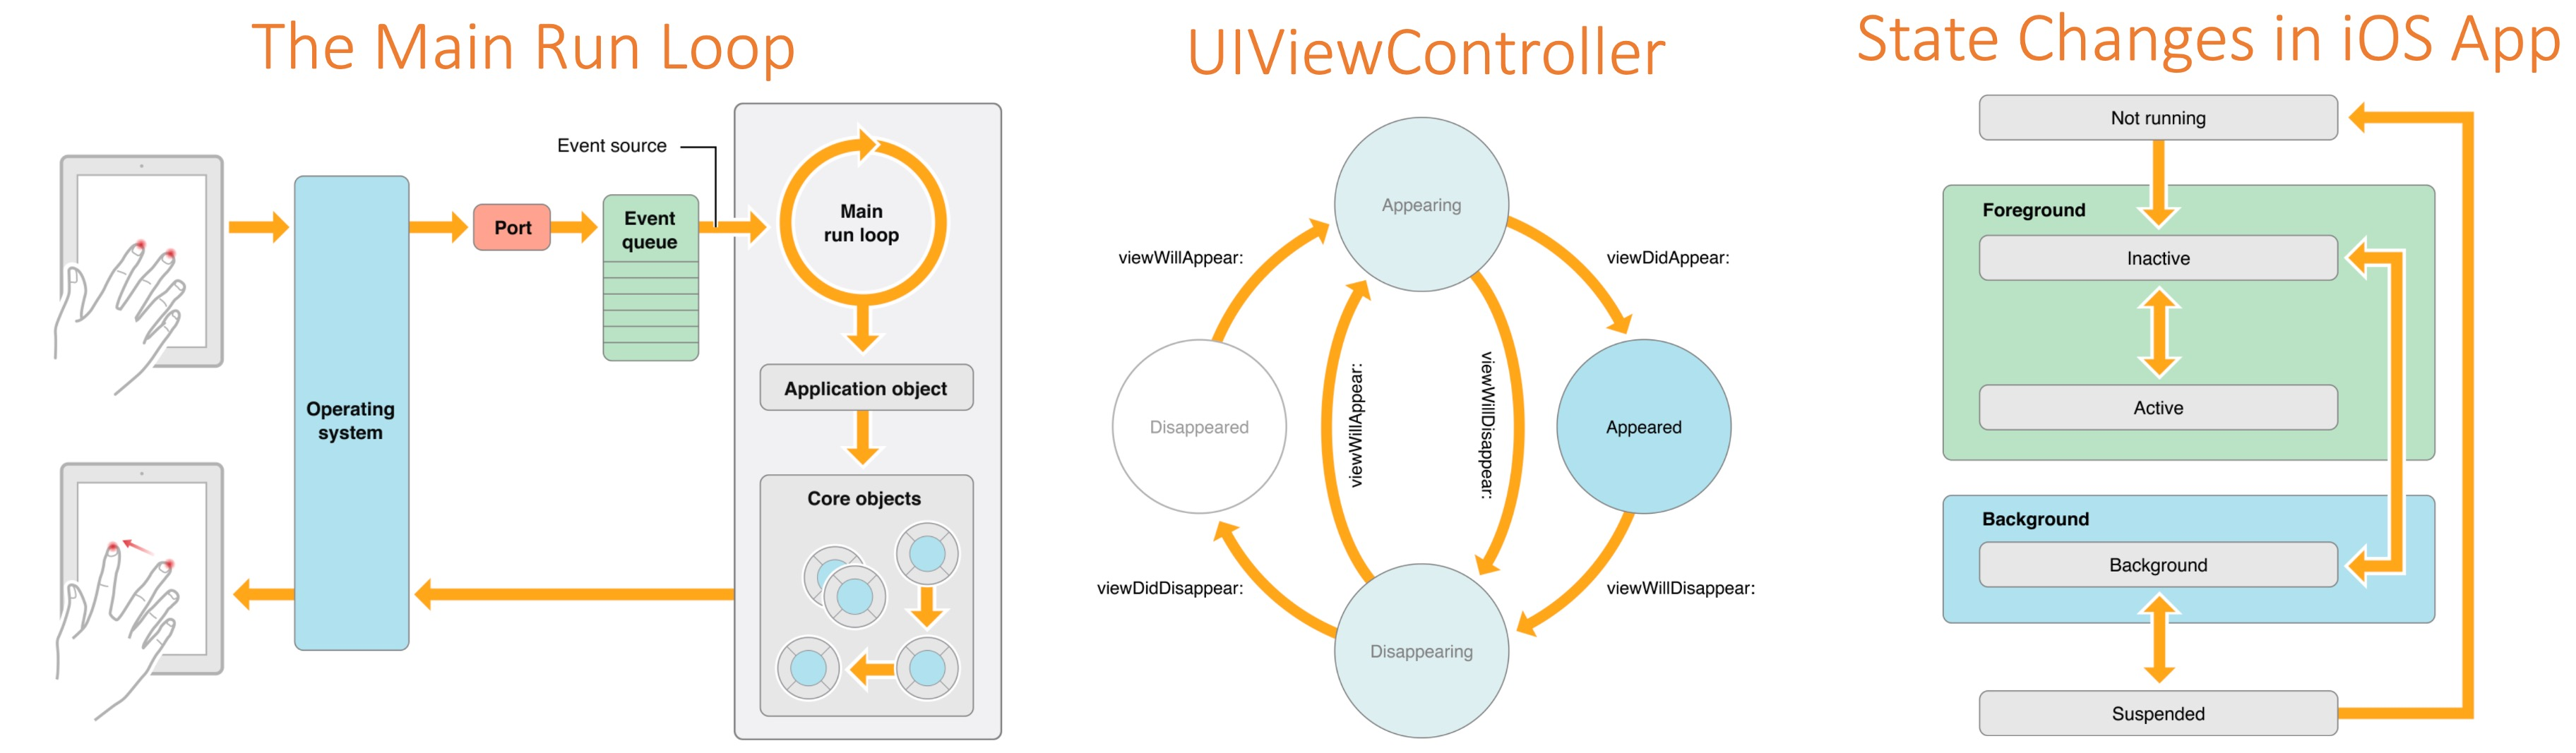
\includegraphics[width=1\linewidth]{appLifecycle.jpg}}

\subsection{UIViewController Lifecycle (Push ViewController A $\rightarrow$ VC B): Entry Process}
\begin{itemize}
  \item Lifecycle stages are predictable and should be used intentionally.
  \item \textbf{init / initWithCoder}: allocate resources and receive dependencies.
  \item \textbf{awakeFromNib}: nib loaded, outlets not fully laid out.
  \item \textbf{loadView}: create view hierarchy (override only if building UI in code).
  \item \textbf{prepareForSegue}: pass data before transition.
  \item \textbf{viewDidLoad}: called once; outlets connected; good for one-off setup or background work.
  \item \textbf{viewWillAppear}: called every time view appears; restart tasks that must be fresh.
  \item \textbf{viewWill/DidLayoutSubviews}: layout pass (constraints resolved).
  \item \textbf{viewDidAppear}: start animations, media, or data fetching.
  \item \textbf{didMoveToParentViewController}: completes parent-child transition.
\end{itemize}

\subsection{UIViewController Lifecycle (Push VC B $\rightarrow$ VC C): B Exit Process}
\begin{itemize}
  \item \textbf{prepareForSegue}: trigger transition and pass data. (Segue: uninterrupted transition)
  \item \textbf{viewWillDisappear}: about to leave screen.
  \item \textbf{viewDidDisappear}: stop timers, notifications, sensors.
  \item \textbf{didReceiveMemoryWarning}: notifies low memory. release caches if possible.
  \item \textbf{deinit}: final cleanup before deallocation.
\end{itemize}

\subsection{\underline{Why Use Asynchronous?}}
\begin{itemize}
  \item \textbf{UI responsiveness}: long tasks on the main thread freeze UI.
  \item \textbf{Parallelism}: iOS devices have multiple cores; concurrent work can use them.
  \item \textbf{But}: concurrency is hard to reason about, costly to debug, and can slow code if abused.
\end{itemize}

\subsection{Concurrency Pitfalls}
\begin{itemize}
  \item \textbf{Race conditions}: order of execution is not deterministic.
  \item \textbf{Reordering}: compiler or CPU may reorder instructions unless constrained.
  \item Result: counter-intuitive outcomes (e.g. two threads both reading old values).
\end{itemize}

\begin{verbatim}
// Thread 1            // Thread 2
x = 1                  r1 = y
y = 1                  r2 = x
// Possible: r1 = 0, r2 = 0 (init values as 0)
\end{verbatim}

\subsection{Threads vs Tasks}
\begin{itemize}
  \item \textbf{Thread}: a path of execution that shares memory with others.
  \item \textbf{Task}: abstract unit of work (often a closure in Swift).
  \item Avoid manual thread management (NSThread) unless absolutely necessary.
\end{itemize}

\subsection{Critical Sections and Methods of Synchronisation}
\begin{itemize}
  \item \textbf{Critical section}: code that must not run concurrently.
  \item \textbf{Techniques}: atomic operations, memory barriers, volatile variables, locks.
  \item Swift provides limited low-level primitives; prefer higher-level frameworks.
\end{itemize}

\begin{verbatim}
// Non-atomic increment, vs Atomic (C / legacy APIs)
x += 1
OSAtomicIncrement32(&x)
\end{verbatim}


\subsection{Locks and Semaphores}
\begin{itemize}
  \item \textbf{Locks / mutexes}: mutual exclusion for critical sections.
  \item Variants: re-entrant, unfair, spin locks (tradeoffs in fairness vs latency).
  \item \textbf{Semaphores}: counting lock; used for producer-consumer.
  \item Pitfalls: accidental release, recursive deadlock, task-death deadlock, priority inversion.
\end{itemize}

\subsection{Grand Central Dispatch (GCD) - fancy name for libdispatch}
\begin{itemize}
  \item GCD is the primary concurrency framework (libdispatch).
  \item In Swift, tasks to be carried out are closures, or function pointers, submitted to dispatch queues. GCD will call up a thread to service that task, tear down the thread when done.
  \item GCD handles thread pool management, scheduling, and context switching.
  \item \textbf{Dispatch queues} run tasks (closures).
  \item \textbf{Serial queue}: one task at a time. \textbf{Concurrent queue}: tasks start FIFO but run in parallel.
  \item \textbf{Two ways of dispatch}: \textbf{async}: submit work, return immediately. \textbf{sync}: submit work, block.
\end{itemize}

\subsection{Types of Queues}
\begin{itemize}
  \item \textbf{Main queue}: serial, runs on main thread.
  \item \textbf{Global Background queues}: concurrent, QoS-based (high/default/low/background).
  \item \textbf{Custom queues}: serial or concurrent; ends up in one of global pools.
\end{itemize}

\subsection{Quality of Service (QoS)}
\begin{itemize}
  \item use QoS to indicate task priority and resource needs, instead of priority, specified for tasks.
  \item \textbf{User-interactive}: immediate UI work, usually on main thread.
  \item \textbf{User-initiated}: user waiting, high priority.
  \item \textbf{Utility}: long-running work, energy efficient.
  \item \textbf{Background}: maintenance, prefetching. Tasks users not aware of.
  \item High QoS task will elevate queued tasks.
\end{itemize}

In Application Main Thread, has a main run loop that processes events and schedules work. The main dispatch queue is serial, runs on the main thread; only main thread can update UI.

\subsection{Handling Events Asynchronously}
\begin{itemize}
  \item Do heavy work off the main thread, then return to main queue for UI updates.
\end{itemize}

\begin{verbatim}
let queue = DispatchQueue(label: "com.example.app")
queue.async {
  let smallImage = image.resize(to: rect)
  DispatchQueue.main.async {
    imageView.image = smallImage
  }
}
\end{verbatim}

\subsection{Structuring Concurrent Work in Applications}
\begin{itemize}
  \item Split by subsystems (UI, data transform, networking, database).
  \item Use queues per subsystem and keep data flow explicit.
  \item \textbf{Chaining}: tasks depend on previous tasks. \textbf{Grouping}: tasks run in parallel then join.
\end{itemize}

\subsection{Dispatch Groups and Work Items}
\begin{itemize}
  \item \textbf{DispatchGroup}: track multiple tasks; use \texttt{notify} to join.
  \item \textbf{DispatchWorkItem}: attach flags, QoS, or cancellation behavior.
\end{itemize}

\begin{verbatim}
let group = DispatchGroup()
queue.async(group: group) { ... }
group.notify(queue: DispatchQueue.main) { ... }
\end{verbatim}

\subsection{Controlling Concurrency}
\begin{itemize}
  \item Too many concurrent tasks can cause \textbf{thread explosion}.
  \item Prefer async APIs and limit concurrency (serial queues, operation queues).
  \item \textbf{sync} on main or same queue risks deadlock.
\end{itemize}

\subsection{Dispatch Barriers}
\begin{itemize}
  \item Dispatch Barriers allow you to make a concurrent queue act like a serial queue for a specific task. Wait for all previously submitted tasks to finish, then execute the barrier task exclusively, then allow subsequent tasks to proceed concurrently.
  \item Use on concurrent queues to isolate a write among reads. (Protect writes to shared data while allow concurrent reads). Gives reader-writer pattern without locks.
  \item Best used on a custom concurrent queue.
\end{itemize}

\subsection{Swift Concurrency (Swift 5.5+)}
\begin{itemize}
  \item \textbf{async/await}: use async for functions, await marks suspension points explicitly.
  \item Asynchronous functions can only be called from other async contexts, \texttt{@main}, or child tasks.
  \item \textbf{Task}: unstructured child task with a handle for results. Allows you to call async API in synchronous code. (Wrap it in a Task, don't await, fire and forget).
  \begin{verbatim}
  func listPhotos(inGallery name: String) async -> [String] { ... }
  let names = await listPhotos(inGallery: "Summer")

  // unstructured child task, not tied to parent tasks lifetime
  let handle = Task {
    return await add(newPhoto, toGalleryNamed: "Spring")
  }
  let result = await handle.value
  \end{verbatim}
  \item \textbf{Actors}: isolate mutable state; only one task can access actor mutable state at a time.
  \begin{verbatim}
  actor TemperatureLogger {
    let label: String
    var measurements: [Int]
    private(set) var max: Int

    init(label: String, measurement: Int) {
      self.label = label
      self.measurements = [measurement]
      self.max = measurement }
  }

  let logger = TemperatureLogger(label: "Outdoors", measurement: 25)
  print(await logger.max) // access may suspend execution
  \end{verbatim}
  \item \textbf{Async sequences}: iterate values over time with \texttt{for try await}.
\end{itemize}
\begin{verbatim}
async let first = downloadPhoto(named: photoNames[0])
async let second = downloadPhoto(named: photoNames[1])
let photos = await [first, second]
\end{verbatim}

\subsection{Object Lifecycle in a Concurrent World}
\begin{itemize}
  \item Lifecycle pattern: \textbf{setup} $\rightarrow$ \textbf{activate} $\rightarrow$ \textbf{invalidate} $\rightarrow$ \textbf{deallocate}.
  \item Use explicit invalidation to unregister observers safely before deinit.
  \item Guard callbacks after invalidation to avoid races or use-after-free.
  \item \textbf{Why explicit invalidation?} Observers are often retained by the subsystem; unregistering in \texttt{deinit} can run on the wrong queue and cause deadlocks or leave references behind (leaks).
  \item \textbf{Rule of thumb}: invalidate on the correct queue (often main), then allow deallocation to happen later on a single thread.
  \item \textbf{In-flight callbacks}: even after unregistering, a callback may already be queued; check an \texttt{invalidated} flag in handlers.
\end{itemize}

\begin{verbatim}
class BusyController: SubsystemObserving {
  private var invalidated = false

  func invalidate() {
    dispatchPrecondition(.onQueue(DispatchQueue.main))
    invalidated = true
    DataTransform.sharedInstance.unregister(observer: self)
  }

  func systemStarted(...) {
    if invalidated { return }
    ...
  }

  deinit { precondition(invalidated) }
}
\end{verbatim}

\subsection{Summary}
\begin{itemize}
  \item Concurrency is powerful but risky; use frameworks and patterns.
  \item Dispatch queues make concurrency manageable, Swift 5.5+ makes it safer.
  \item Prefer clear lifecycle and explicit invalidation in concurrent observer designs.
\end{itemize}

\columnbreak

\section{Lecture 5: Entity Component Systems (ECS)}

\subsection{Why ECS for Game Architecture?}
\begin{itemize}
  \item Games have tight frame budgets and a \textbf{game loop} with ordered, repeated updates.
  \item OOP/POP often lead to deep hierarchies or tangled compositions when behaviors combine.
  \item ECS separates \textbf{data (components)} from \textbf{behavior (systems)} to scale complexity.
\end{itemize}

\begin{verbatim}
void update(int time) {
  game.update(time);
  spaceship.updateInputs(time);
  foreach (Enemy e : enemies) spaceship.move(time);
  foreach (Enemy e : enemies)
    foreach (Bullet b : bullets) collisionManager.update(time);
  spaceship.render(canvas);
  foreach (Enemy e : enemies) foreach (Obstacle o : obstacles) ...
  e.updateAI(time);
  e.move(time);
  b.move(time);
  e.render(canvas);
  o.render(canvas);
}
\end{verbatim}

\subsection{Process-Oriented Loop}
\begin{itemize}
  \item Use processes to break the loop into manageable stages (render, move, AI, collision).
  \item The command/process manager orders updates by priority.
  \item \textbf{Intuitive and good}: mirrors how humans think about game stages.
  \item \textbf{But}: still process-centric, can hard-code entity lists and duplicate data; ECS refines this by separating data (components) from behavior (systems).
\end{itemize}

\begin{verbatim}
interface IProcess {
  bool start();
  void update(int time);
  void stop();
}

class ProcessManager {
  private PriorityQueue<Process> processes = new PriorityQueue ...
  bool addProcess(Process process, int priority) { ... }
  void update(int time) { foreach(Process p : processes) p.update(time); }
  void removeProcess(Process process) { ... }
}
\end{verbatim}

\subsection{Example: Rendering as a Process}
\begin{itemize}
  \item Introduce \texttt{IRenderable} so the renderer depends on capability, not concrete types.
  \item Avoids hard-coding entity lists in rendering logic.
  \item \textbf{Why here?}  Concrete example of splitting the big game loop into focused
  processes and shows dependency inversion: the render stage depends on an interface, not entities.
\end{itemize}

\begin{verbatim}
interface IRenderable { void render(Canvas canvas); }

class RenderProcess implements IProcess {
  private Canvas canvas;
  private Vector<IRenderable> renderables;
  void update(int time) {
    foreach(IRenderable r : renderables) r.render(canvas);
  }
}
\end{verbatim}

\subsection{Issue: Having to use an Inheritance Chain}
\begin{itemize}
  \item \textbf{DRY via base class} helps reuse (Renderable), but combining behaviors leads to
  multiple inheritance or awkward chains.
  \item Example problem: a \texttt{Movable} that is not \texttt{Renderable}.
  \item \textbf{BAD}: inheritance forces unrelated capabilities into one hierarchy, make types bloated, brittle.
  \item \textbf{BAD}: adding a new behavior can ripple through the whole tree (fragile base class).
\end{itemize}

\begin{verbatim}
class Renderable implements IRenderable { ... }
class Movable implements IMovable { ... }
class Spaceship extends Movable, Renderable { } 
// not possible in most OO langs
\end{verbatim}

\subsection{Issue: What about Composition Over Inheritance?}
\begin{itemize}
  \item Compose behavior via delegates, but shared data becomes tricky (position, rotation).
  \item Interfaces alone provide methods, not shared state; you end up duplicating fields.
  \item \textbf{BAD}: duplicated state across delegates causes divergence bugs (render position $\neq$ move position).
  \item \textbf{OK}: composition avoids hierarchy explosion but still lacks a shared data model.
\end{itemize}

\begin{verbatim}
class Spaceship implements IRenderable, IMovable {
  Renderable renderDelegate;
  Movable moveDelegate;
  func render(canvas) { renderDelegate.render(canvas); }
  func move(time) { moveDelegate.move(time); }
}
\end{verbatim}

\subsection{Swift Semantics: Protocols Help, But Still Tight}
\begin{itemize}
  \item Swift protocols can require properties + default implementations.
  \item Still forces each entity to carry all fields for every capability.
  \item \textbf{BAD}: entity types grow as you add capabilities; unused fields are carried around.
  \item \textbf{BAD}: coupling between data and behavior remains at the entity level.
\end{itemize}

\begin{verbatim}
protocol Renderable {
  var sprite: Sprite { get set }
  var position: Point { get set }
  var rotation: Double { get set }
  func render(canvas: Canvas) -> ()
}
\end{verbatim}

\subsection{Architectural Pattern: Use Components}
\begin{itemize}
  \item Split state into small, reusable components.
  \item Entities are just IDs with a set of components.
  \item \textbf{GOOD}: data is normalized; no duplication between systems.
  \item \textbf{GOOD}: features are additive (add/remove components without changing types).
\end{itemize}

\begin{verbatim}
struct PositionComponent { var x: Double; var y: Double; 
                            var rotation: Double }
struct VelocityComponent { var velocityX: Double; var velocityY: Double; 
                            var angularVelocity: Double }
struct SpriteComponent { var sprite: Sprite }
\end{verbatim}

\subsection{Systems (formerly Processes)}
\begin{itemize}
  \item Systems operate on \textbf{sets of components}, not concrete entities.
  \item RenderSystem needs Position + Sprite; MoveSystem needs Position + Velocity.
  \item This avoids inheritance, favors data-oriented design, and is cache-friendly.
  \item \textbf{GOOD}: behavior scales with combinations of components, not class hierarchies.
  \item \textbf{GOOD}: easy to introduce new systems without touching entity definitions.
\end{itemize}

\begin{verbatim}
class RenderSystem: System {
  var renderables: [RenderData]
  func update(time: Int) {
    renderables.forEach { r in
      canvas.draw(r.sprite.sprite, 
                  r.position.x, r.position.y, 
                  r.position.rotation)
    }
  }
}
\end{verbatim}

\subsection{Steps to transition From Processes to Systems (Entity Component Systems)}
\begin{itemize}
  \item Start with data classes per process (\texttt{RenderData}, \texttt{MoveData}) $\rightarrow$ breaks encapsulation.
  \item Remove data classes; systems operate directly on components.
  \item Rename processes to \textbf{systems} once they are pure component processors.
  \item Entities become just \textbf{bags of components}.
\end{itemize}

\subsection{Entity Explosion and Querying}
\begin{itemize}
  \item Entities can be created by assembling components at runtime.
  \item A \texttt{Nexus} (world) tracks entities and systems; systems query by component sets.
  \item Tradeoff: more indirection, but much more flexible composition.
  \item \textbf{Nexus as ECS extension}: centralizes storage, indexing, and scheduling so systems stay pure.
  \item \textbf{Why it helps}: avoids passing huge lists everywhere; queries become ``give me all entities with Position+Velocity''.
  \item \textbf{Implementation intuition}: often a dictionary/map from entity IDs to component sets (or component type to entity data); high-performance ECS may use arrays/archetypes instead.
\end{itemize}

\begin{verbatim}
class Entity { var components = Set<Components>() }

class Nexus {
  var entities = Dictionary<UUID, [Components]>()
  var systems = PriorityQueue<System>()
  func getEntities(with components: [Components]) -> [[Components]] { ... }
  func update(time: Int) { systems.forEach { $0.update(time, self) } }
}
\end{verbatim}

\subsection{Summary}
\begin{itemize}
  \item ECS separates \textbf{entities} (IDs), \textbf{components} (data), and \textbf{systems} (logic).
  \item Great for games where behavior mixes combinatorially and performance matters.
  \item Costs: more plumbing and less encapsulation; use when flexibility outweighs that cost.
\end{itemize}


\vfill \null
\columnbreak


\section{Lecture D: Protocol Oriented Programming}

\subsection{Why POP? What about OOP?}
\begin{itemize}
  \item OOP strengths: \textbf{encapsulation}, access control, abstraction, namespaces (logical grouping no name conflicts), expressive syntax, extensibility.
  \item Inheritance - reuse complex logic, allow overrides, but large hierarchies often become brittle.
  \item Most real systems want \textbf{composition} rather than deep inheritance trees.
\end{itemize}

\subsection{Why Inheritance Hurts}
\begin{itemize}
  \item \textbf{Intrusive inheritance}: only one superclass; must inherit its stored properties and init rules.
  \item \textbf{Implicit sharing}: references lead to surprising mutations, defensive copying, locks, bugs.
  \item \textbf{Lost type relationships}: base types erase concrete info, forcing casts and runtime checks.
\end{itemize}

\begin{verbatim}
class Ordered {
  func precedes(other: Ordered) -> Bool { fatalError("Implement me!") }
}
class Number: Ordered {
  var value: Double = 0
  override func precedes(other: Ordered) -> Bool {
    return value < (other as! Number).value // forced downcast
  }
}
\end{verbatim}

\subsection{Protocol-Oriented Programming}
\begin{itemize}
  \item Start with a \textbf{protocol} before writing a class; model behavior instead of hierarchy.
  \item Use \textbf{value types} (structs) when possible to avoid implicit sharing.
\end{itemize}

\begin{verbatim}
protocol Ordered {
  // Self requirement: same concrete type as me
  func precedes(other: Self) -> Bool
}

struct Number: Ordered {
  var value: Double = 0
  func precedes(other: Number) -> Bool { value < other.value }
}
\end{verbatim}

\subsection{Two Worlds of Protocols}
\begin{itemize}
  \item \textbf{Without Self}: usable as a type (existential), heterogeneous collections, dynamic dispatch. Every model must deal with all others. Less optimisable.
  \item \textbf{With Self}: only usable as a generic constraint, homogeneous collections (all same type that implements protocol), static dispatch.
\end{itemize}

\begin{verbatim}
// Heretogeneous, cannot work with self (can't precedes() across types)
func binarySearch(sortedKeys: [Ordered], forKey k: Ordered) -> Int { ... }

// Generic, homogeneous
func binarySearch<T: Ordered>(sortedKeys: [T], forKey k: T) -> Int { ... }
\end{verbatim}

\subsection{Renderer Example (Protocols + Generics)}
\begin{itemize}
  \item Define \texttt{Drawable} and a \texttt{Renderer} protocol to separate drawing intent from rendering backend.
  \item Enables testing via a \texttt{TestRenderer} and real rendering via CoreGraphics.
  \item \textbf{Retroactive modeling}: extend existing types to conform without modifying them.
\end{itemize}

\begin{verbatim}
protocol Renderer {
  func moveTo(position: CGPoint)
  func lineTo(position: CGPoint)
  func arcAt(center: CGPoint, radius: CGFloat,
             startAngle: CGFloat, endAngle: CGFloat)
}

protocol Drawable { func draw(renderer: Renderer) }

struct Circle: Drawable { ... }
struct Polygon: Drawable { ... }

// extend Swift's CGContext to conform to Renderer
extension CGContext: Renderer { ... } // retroactive modeling
\end{verbatim}

\subsection{Protocol Extensions}
\begin{itemize}
  \item Provide \textbf{default implementations} and new APIs without changing conforming types.
  \item Extensions can be \textbf{constrained} (e.g., only when \texttt{Self: Equatable}).
  \item Customization points: default behavior can be overridden by conforming types.
\end{itemize}

\begin{verbatim}
extension Renderer {
  func circleAt(center: CGPoint, radius: CGFloat) {
    arcAt(center: center, radius: radius, startAngle: 0, endAngle: twoPi)
  }
}

extension Ordered where Self: Comparable {
  func precedes(other: Self) -> Bool { self < other }
}
\end{verbatim}

\subsection{Bridging Heterogeneous Types}
\begin{itemize}
  \item Protocols with \texttt{Self} cannot be used as heterogeneous element types.
  \item Bridge with a type-erased method (e.g., \texttt{isEqualTo}) to compare different \texttt{Drawable}s.
\end{itemize}

\begin{verbatim}
protocol Drawable {
  func draw(renderer: Renderer)
  func isEqualTo(other: Drawable) -> Bool
}
extension Drawable where Self: Equatable {
  func isEqualTo(other: Drawable) -> Bool {
    if let o = other as? Self { return self == o }
    return false
  }
}
\end{verbatim}

\subsection{Generics vs Associated Types}
\begin{itemize}
  \item \textbf{Generics}: define a concrete implementation over a type parameter.
  \item \textbf{Generics expand implementation}: a generic function/type is one implementation that works for many types.
  \item \textbf{Associated types}: protocols specify placeholders to be filled by conforming types.
  \item \textbf{Associated types expand vocabulary}: a protocol is a checklist of requirements plus a named type slot. (A protocol with a 'type' slot.)
\end{itemize}

\begin{verbatim}
  // Associated type
  protocol Container {
    associatedtype T
    mutating func append(_ item: T)
    var count: Int { get }
    subscript(i: Int) -> T { get }
  }

  // Associated types filled by conformers
  class BagOfBytes: Container {
    func append(_ item: UInt8) { ... }
    subscript(i: Int) -> UInt8 { ... }
  }

  struct BunchOfEquatables<T: Equatable>: Container {
    func append(_ item: T) { ... }
    subscript(i: Int) -> T { ... }
  }

  // Generic struct
  struct Stack<T>: Container { ... }

  // Generic type parameters (one implementation, many types)
  class ViewController<V: View> { var view: V }

  func allEqual<T: Equatable>(a: T, b: T, c: T) -> Bool {
    return a == b && b == c
  }
\end{verbatim}

\subsection{When to Use Classes}
\begin{itemize}
  \item Use classes when implicit sharing is desired or required by frameworks.
  \item Examples: UI objects, file handles, sinks to external state (e.g., \texttt{CGContext}).
  \item Don't fight the system, if a framework expects a class, use a class. On the other hand, be circumspect, nothing should grow too large, when factoring something out of a class, consider making it a struct + protocol instead.
  \item Otherwise, prefer structs + protocols for composition and testability.
\end{itemize}

\subsection{Swift Protocols vs Java Interfaces}
\begin{itemize}
  \item Swift protocols can require initializers, static methods, operators, and subscripts.
  \item Conditional conformances and constrained extensions enable expressive reuse.
  \item Default implementations and retroactive modeling support composition over inheritance.
\end{itemize}

\subsection{Composition Over Inheritance}
\begin{itemize}
  \item Protocols as composition: Favor small, focused protocols over large monolithic ones.
  \item Avoid ``god classes'' by splitting features into protocols and delegates.
  \item Use adapters/decorators/proxies to compose behavior without inheritance chains.
\end{itemize}

\subsection{Summary}
\begin{itemize}
  \item Protocols + value types + extensions are the core of Swift POP.
  \item Prefer composition and generic constraints to reduce hierarchy complexity.
  \item Use classes intentionally when identity and shared mutable state are essential.
\end{itemize}

\vfill \null

\columnbreak

\section{Lecture E: Errors and Exceptions}

\subsection{Context and History}
\begin{itemize}
  \item Cocoa / Objective-C legacy influences Swift error handling (type bridging, NSError APIs).
  \item Objective-C initially lacked native exceptions; \texttt{NSException} was added via macros and reserved for catastrophic, unrecoverable errors.
  \item \texttt{NSError} predates exceptions and is used for recoverable, user-facing failures.
\end{itemize}

\subsection{Errors vs Exceptions}
\begin{itemize}
  \item \textbf{NSError}: recoverable, expected failures (e.g., file not found).
  \item \textbf{NSException}: programmer/runtime errors (e.g., out-of-bounds), not meant for control flow.
  \item Swift introduces \textbf{Error} and \textbf{throw/try/catch} with explicit handling.
\end{itemize}

\subsection{Swift Error Handling}
\begin{itemize}
  \item \textbf{Define}: create error types conforming to \texttt{Error}.
  \item \textbf{Throw}: mark functions with \texttt{throws}.
  \item \textbf{Handle}: use \texttt{do-try-catch}, \texttt{try?}, or \texttt{try!}.
  \item \textbf{Propagate}: a function can \texttt{throws} if it only fails when a callee fails.
\end{itemize}

\begin{verbatim}
enum FileError: Error { case notFound, unreadable }

func load(path: String) throws -> Data { ... }

do {
  let data = try load(path: "notes.txt")
} catch {
  // handle
}
\end{verbatim}

\subsection{Handling Options}
\begin{itemize}
  \item \textbf{do-try-catch}: explicit recovery paths.
  \item \textbf{try?}: converts errors to \texttt{nil} (optional result).
  \item \textbf{try!}: disables error handling; crashes if an error is thrown.
  \item \textbf{defer}: runs cleanup code on exit, even with errors.
\end{itemize}

\subsection{Checked vs Unchecked}
\begin{itemize}
  \item Java has checked and unchecked exceptions.
  \item Swift has no unchecked exceptions; all \texttt{throw} sites must be acknowledged.
  \item Runtime traps (e.g., out-of-bounds) still exist and terminate execution.
\end{itemize}

\subsection{Why Not Special Return Values?}
\begin{itemize}
  \item Special values are ambiguous and may collide with valid results.
  \item They carry limited error information unless wrapped in a custom type.
  \item Swift errors are effectively \textbf{typed return values} with syntactic sugar.
\end{itemize}

\subsection{Performance Notes}
\begin{itemize}
  \item Exceptions are expensive in many languages due to stack unwinding and binary bloat.
  \item Swift favors explicit error paths over hidden runtime costs.
\end{itemize}

\subsection{Interacting with Cocoa}
\begin{itemize}
  \item Swift bridges to Objective-C APIs that use \texttt{NSErrorPointer}.
  \item Swift 2.0 introduced automatic conversion of many Cocoa APIs to \texttt{throws}.
  \item Legacy APIs still expose \texttt{NSError} and must be handled explicitly.
\end{itemize}

\subsection{Summary}
\begin{itemize}
  \item Swift error handling is explicit, typed, and recoverable.
  \item Exceptions are for programmer errors; use \texttt{Error} for expected failures.
  \item Cocoa legacy shapes the API surface; bridging is common in real codebases.
\end{itemize}

\columnbreak

\section{Lecture F: Requirements and Specifications}

\subsection{Motivation: Requirements Drive Design}
\begin{itemize}
  \item A game engine focuses on gameplay logic and state; a physics engine focuses on motion and collision.
  \item Requirements shape decomposition: model/view/controller vs physics subsystems.
  \item Composition (protocols/decorators) can avoid rigid inheritance as features like gravity, forces, or special effects grow.
\end{itemize}

\subsection{Why Requirements Matter}
\begin{itemize}
  \item Wrong requirements and late integration are expensive to fix.
  \item Requirements change; plan for evolution rather than locking into a brittle design.
  \item Users often cannot articulate needs directly; you must uncover the real problem.
\end{itemize}

\subsection{Software Development Life Cycle (SDLC)}
\begin{itemize}
  \item \textbf{Waterfall}: sequential phases; clear milestones but rigid to change.
  \item \textbf{Spiral}: iterate with risk analysis; suitable for high-uncertainty projects.
  \item \textbf{Agile}: iterative, incremental delivery with frequent feedback loops.
\end{itemize}

\subsection{Requirements Analysis}
\begin{itemize}
  \item Understand workflow and user interactions; remember users do not think like developers.
  \item Consider failure modes: what happens when things go wrong?
  \item Capture \textbf{functional} requirements, \textbf{performance} constraints, and \textbf{delivery} schedule.
\end{itemize}

\subsection{Specifications and Diagrams}
\begin{itemize}
  \item Specifications define operations and constraints for static or running systems.
  \item Diagrams clarify structure: ERD for entities/relations, MDD for class/module interactions.
  \item A picture can surface missing constraints earlier than prose alone.
\end{itemize}

\subsection{Design Goals and Decomposition}
\begin{itemize}
  \item Aim for modular structure with clear abstractions and independent implementations.
  \item Decompose to reduce complexity, divide work, improve flexibility and reuse.
  \item Prefer high cohesion and low coupling; use design patterns to guide interfaces.
\end{itemize}

\subsection{Interfaces vs Implementation}
\begin{itemize}
  \item A module's API is the contract; implementation can change without breaking clients.
  \item Phased implementation helps manage scope: build in small, testable increments.
  \item Design for change: think big, implement in small steps.
\end{itemize}

\subsection{Final Project Guidance}
\begin{itemize}
  \item Focus on software engineering, not just flashy features.
  \item Plan: data model, design (ERD/MDD), specifications, and usability.
  \item Implement with ADTs, clear dependencies, unit tests, and staged integration.
  \item Requirements may change midstream; reconcile external needs with course goals.
\end{itemize}

\end{multicols*}
\end{document}
